% Options for packages loaded elsewhere
\PassOptionsToPackage{unicode}{hyperref}
\PassOptionsToPackage{hyphens}{url}
\PassOptionsToPackage{dvipsnames,svgnames,x11names}{xcolor}
%
\documentclass[
  letterpaper,
  DIV=11,
  numbers=noendperiod]{scrartcl}

\usepackage{amsmath,amssymb}
\usepackage{iftex}
\ifPDFTeX
  \usepackage[T1]{fontenc}
  \usepackage[utf8]{inputenc}
  \usepackage{textcomp} % provide euro and other symbols
\else % if luatex or xetex
  \usepackage{unicode-math}
  \defaultfontfeatures{Scale=MatchLowercase}
  \defaultfontfeatures[\rmfamily]{Ligatures=TeX,Scale=1}
\fi
\usepackage{lmodern}
\ifPDFTeX\else  
    % xetex/luatex font selection
\fi
% Use upquote if available, for straight quotes in verbatim environments
\IfFileExists{upquote.sty}{\usepackage{upquote}}{}
\IfFileExists{microtype.sty}{% use microtype if available
  \usepackage[]{microtype}
  \UseMicrotypeSet[protrusion]{basicmath} % disable protrusion for tt fonts
}{}
\makeatletter
\@ifundefined{KOMAClassName}{% if non-KOMA class
  \IfFileExists{parskip.sty}{%
    \usepackage{parskip}
  }{% else
    \setlength{\parindent}{0pt}
    \setlength{\parskip}{6pt plus 2pt minus 1pt}}
}{% if KOMA class
  \KOMAoptions{parskip=half}}
\makeatother
\usepackage{xcolor}
\setlength{\emergencystretch}{3em} % prevent overfull lines
\setcounter{secnumdepth}{-\maxdimen} % remove section numbering
% Make \paragraph and \subparagraph free-standing
\makeatletter
\ifx\paragraph\undefined\else
  \let\oldparagraph\paragraph
  \renewcommand{\paragraph}{
    \@ifstar
      \xxxParagraphStar
      \xxxParagraphNoStar
  }
  \newcommand{\xxxParagraphStar}[1]{\oldparagraph*{#1}\mbox{}}
  \newcommand{\xxxParagraphNoStar}[1]{\oldparagraph{#1}\mbox{}}
\fi
\ifx\subparagraph\undefined\else
  \let\oldsubparagraph\subparagraph
  \renewcommand{\subparagraph}{
    \@ifstar
      \xxxSubParagraphStar
      \xxxSubParagraphNoStar
  }
  \newcommand{\xxxSubParagraphStar}[1]{\oldsubparagraph*{#1}\mbox{}}
  \newcommand{\xxxSubParagraphNoStar}[1]{\oldsubparagraph{#1}\mbox{}}
\fi
\makeatother

\usepackage{color}
\usepackage{fancyvrb}
\newcommand{\VerbBar}{|}
\newcommand{\VERB}{\Verb[commandchars=\\\{\}]}
\DefineVerbatimEnvironment{Highlighting}{Verbatim}{commandchars=\\\{\}}
% Add ',fontsize=\small' for more characters per line
\usepackage{framed}
\definecolor{shadecolor}{RGB}{241,243,245}
\newenvironment{Shaded}{\begin{snugshade}}{\end{snugshade}}
\newcommand{\AlertTok}[1]{\textcolor[rgb]{0.68,0.00,0.00}{#1}}
\newcommand{\AnnotationTok}[1]{\textcolor[rgb]{0.37,0.37,0.37}{#1}}
\newcommand{\AttributeTok}[1]{\textcolor[rgb]{0.40,0.45,0.13}{#1}}
\newcommand{\BaseNTok}[1]{\textcolor[rgb]{0.68,0.00,0.00}{#1}}
\newcommand{\BuiltInTok}[1]{\textcolor[rgb]{0.00,0.23,0.31}{#1}}
\newcommand{\CharTok}[1]{\textcolor[rgb]{0.13,0.47,0.30}{#1}}
\newcommand{\CommentTok}[1]{\textcolor[rgb]{0.37,0.37,0.37}{#1}}
\newcommand{\CommentVarTok}[1]{\textcolor[rgb]{0.37,0.37,0.37}{\textit{#1}}}
\newcommand{\ConstantTok}[1]{\textcolor[rgb]{0.56,0.35,0.01}{#1}}
\newcommand{\ControlFlowTok}[1]{\textcolor[rgb]{0.00,0.23,0.31}{\textbf{#1}}}
\newcommand{\DataTypeTok}[1]{\textcolor[rgb]{0.68,0.00,0.00}{#1}}
\newcommand{\DecValTok}[1]{\textcolor[rgb]{0.68,0.00,0.00}{#1}}
\newcommand{\DocumentationTok}[1]{\textcolor[rgb]{0.37,0.37,0.37}{\textit{#1}}}
\newcommand{\ErrorTok}[1]{\textcolor[rgb]{0.68,0.00,0.00}{#1}}
\newcommand{\ExtensionTok}[1]{\textcolor[rgb]{0.00,0.23,0.31}{#1}}
\newcommand{\FloatTok}[1]{\textcolor[rgb]{0.68,0.00,0.00}{#1}}
\newcommand{\FunctionTok}[1]{\textcolor[rgb]{0.28,0.35,0.67}{#1}}
\newcommand{\ImportTok}[1]{\textcolor[rgb]{0.00,0.46,0.62}{#1}}
\newcommand{\InformationTok}[1]{\textcolor[rgb]{0.37,0.37,0.37}{#1}}
\newcommand{\KeywordTok}[1]{\textcolor[rgb]{0.00,0.23,0.31}{\textbf{#1}}}
\newcommand{\NormalTok}[1]{\textcolor[rgb]{0.00,0.23,0.31}{#1}}
\newcommand{\OperatorTok}[1]{\textcolor[rgb]{0.37,0.37,0.37}{#1}}
\newcommand{\OtherTok}[1]{\textcolor[rgb]{0.00,0.23,0.31}{#1}}
\newcommand{\PreprocessorTok}[1]{\textcolor[rgb]{0.68,0.00,0.00}{#1}}
\newcommand{\RegionMarkerTok}[1]{\textcolor[rgb]{0.00,0.23,0.31}{#1}}
\newcommand{\SpecialCharTok}[1]{\textcolor[rgb]{0.37,0.37,0.37}{#1}}
\newcommand{\SpecialStringTok}[1]{\textcolor[rgb]{0.13,0.47,0.30}{#1}}
\newcommand{\StringTok}[1]{\textcolor[rgb]{0.13,0.47,0.30}{#1}}
\newcommand{\VariableTok}[1]{\textcolor[rgb]{0.07,0.07,0.07}{#1}}
\newcommand{\VerbatimStringTok}[1]{\textcolor[rgb]{0.13,0.47,0.30}{#1}}
\newcommand{\WarningTok}[1]{\textcolor[rgb]{0.37,0.37,0.37}{\textit{#1}}}

\providecommand{\tightlist}{%
  \setlength{\itemsep}{0pt}\setlength{\parskip}{0pt}}\usepackage{longtable,booktabs,array}
\usepackage{calc} % for calculating minipage widths
% Correct order of tables after \paragraph or \subparagraph
\usepackage{etoolbox}
\makeatletter
\patchcmd\longtable{\par}{\if@noskipsec\mbox{}\fi\par}{}{}
\makeatother
% Allow footnotes in longtable head/foot
\IfFileExists{footnotehyper.sty}{\usepackage{footnotehyper}}{\usepackage{footnote}}
\makesavenoteenv{longtable}
\usepackage{graphicx}
\makeatletter
\def\maxwidth{\ifdim\Gin@nat@width>\linewidth\linewidth\else\Gin@nat@width\fi}
\def\maxheight{\ifdim\Gin@nat@height>\textheight\textheight\else\Gin@nat@height\fi}
\makeatother
% Scale images if necessary, so that they will not overflow the page
% margins by default, and it is still possible to overwrite the defaults
% using explicit options in \includegraphics[width, height, ...]{}
\setkeys{Gin}{width=\maxwidth,height=\maxheight,keepaspectratio}
% Set default figure placement to htbp
\makeatletter
\def\fps@figure{htbp}
\makeatother

\usepackage{fvextra}
\DefineVerbatimEnvironment{Highlighting}{Verbatim}{breaklines,commandchars=\\\{\}}

\usepackage{multicol}
\newcommand{\btwocol}{\begin{multicols}{2}}
\newcommand{\etwocol}{\end{multicols}}
\KOMAoption{captions}{tableheading}
\makeatletter
\@ifpackageloaded{caption}{}{\usepackage{caption}}
\AtBeginDocument{%
\ifdefined\contentsname
  \renewcommand*\contentsname{Table of contents}
\else
  \newcommand\contentsname{Table of contents}
\fi
\ifdefined\listfigurename
  \renewcommand*\listfigurename{List of Figures}
\else
  \newcommand\listfigurename{List of Figures}
\fi
\ifdefined\listtablename
  \renewcommand*\listtablename{List of Tables}
\else
  \newcommand\listtablename{List of Tables}
\fi
\ifdefined\figurename
  \renewcommand*\figurename{Figure}
\else
  \newcommand\figurename{Figure}
\fi
\ifdefined\tablename
  \renewcommand*\tablename{Table}
\else
  \newcommand\tablename{Table}
\fi
}
\@ifpackageloaded{float}{}{\usepackage{float}}
\floatstyle{ruled}
\@ifundefined{c@chapter}{\newfloat{codelisting}{h}{lop}}{\newfloat{codelisting}{h}{lop}[chapter]}
\floatname{codelisting}{Listing}
\newcommand*\listoflistings{\listof{codelisting}{List of Listings}}
\makeatother
\makeatletter
\makeatother
\makeatletter
\@ifpackageloaded{caption}{}{\usepackage{caption}}
\@ifpackageloaded{subcaption}{}{\usepackage{subcaption}}
\makeatother

\ifLuaTeX
  \usepackage{selnolig}  % disable illegal ligatures
\fi
\usepackage{bookmark}

\IfFileExists{xurl.sty}{\usepackage{xurl}}{} % add URL line breaks if available
\urlstyle{same} % disable monospaced font for URLs
\hypersetup{
  pdftitle={CS/DS 541: Deep Learning},
  pdfauthor={Tom Arnold \& Nate Hindman},
  colorlinks=true,
  linkcolor={blue},
  filecolor={Maroon},
  citecolor={Blue},
  urlcolor={Blue},
  pdfcreator={LaTeX via pandoc}}


\title{CS/DS 541: Deep Learning}
\usepackage{etoolbox}
\makeatletter
\providecommand{\subtitle}[1]{% add subtitle to \maketitle
  \apptocmd{\@title}{\par {\large #1 \par}}{}{}
}
\makeatother
\subtitle{Homework 3}
\author{Tom Arnold \& Nate Hindman}
\date{}

\begin{document}
\maketitle

\RecustomVerbatimEnvironment{verbatim}{Verbatim}{
  showspaces = false,
  showtabs = false,
  breaksymbolleft={},
  breaklines
  % Note: setting commandchars=\\\{\} here will cause an error
}


\btwocol

\emph{Due: 5:59pm ET Monday September 29}

\emph{This problem can be done in teams of up 2 students.}

\etwocol

\section{Problem 1: Deriving He's initialization {[}10 points + 5 bonus
pts{]}}\label{problem-1-deriving-hes-initialization-10-points-5-bonus-pts}

In Lecture 7, we learned about a widely used technique for setting the
initial values of the weight parameters in a neural network: the
\textbf{He initialization}. Specifically, it samples each weight value
from \(\mathcal{N}(0,2/n_{l})\)---i.e., a 0-mean Gaussian distribution
with variance \(2/n_{l}\) where \(n_{l}\) is the number of columns of
the weight matrix \(W^{[l]}\) layer \(l\) (or, equivalently the
dimension of the inputs fed to layer \(l\)).

Here you are asked to derive some of the steps we skipped in class. We
will start from:
\[Var[z^{[l]}]=Var[w^{[l]}x^{[l]}]=Var[\sum_{j=1}^{n_{l}}w_{j}^{[l]}x_{j}^{[l]}]\]
\[Var[\sum_{j=1}^{n_{l}}w_{j}^{[l]}x_{j}^{[l]}]=n_{l}Var[w_{l}x_{l}],\]

\begin{enumerate}
\def\labelenumi{\arabic{enumi}.}
\tightlist
\item
  (2 points) Explain what are the assumptions that allow us to write:
  \[Var[\sum_{j=1}^{n_{l}}w_{j}^{[l]}x_{j}^{[l]}]=n_{l}Var[w_{l}x_{l}],\]
  where \(w_{l}\) represents any of the \(w_{j}^{[l]}\) weights and
  \(x_{l}\) represents any of the \(x_{j}^{[l]}\) inputs.
\end{enumerate}

\begin{center}\rule{0.5\linewidth}{0.5pt}\end{center}

\subsection{Answer}\label{answer}

We are given that He initialization samples weights from
\(\mathcal{N}(0, 2/n_l)\) which means that each weight has expectation
and variance:

\[E[w_j^{[l]}] = 0 \text{ and } \text{Var}[w_j^{[l]}] = 2/n_l \quad \text{(definition of } \mathcal{N}(\mu, \sigma^2))\]

\[\text{Var}\left[\sum_{j=1}^{n_l} w_j^{[l]} x_j^{[l]}\right] = E\left[\left(\sum_{j=1}^{n_l} w_j^{[l]} x_j^{[l]}\right)^2\right] - \left(E\left[\sum_{j=1}^{n_l} w_j^{[l]} x_j^{[l]}\right]\right)^2\]
\[\text{(Definition of Variance: } \text{Var}[Y] = E[Y^2] - (E[Y])^2)\]

\subsubsection{\texorpdfstring{Assumption 1: \(w_j^{[l]}\) independent
of all
\(x_k^{[l]}\)}{Assumption 1: w\_j\^{}\{{[}l{]}\} independent of all x\_k\^{}\{{[}l{]}\}}}\label{assumption-1-w_jl-independent-of-all-x_kl}

To move forward, we need to assume that the weights \(w_j^{[l]}\) are
independent of the inputs \(x_j^{[l]}\). This assumption allows us to
factor terms of the form
\(E[w_j^{[l]} x_j^{[l]}] = E[w_j^{[l]}] \cdot E[x_j^{[l]}].\) Because we
know from initialization that \(E[w_j^{[l]}] = 0\), the full product is
0 and drops out of the equation.

We are justified in this assumption because the random initialization of
weights at layer \(l\) is done before the network ever sees data, so the
particular input values flowing through the network cannot influence the
weights. Without this assumption, we would have to deal with the full
joint distribution of \((w_j^{[l]}, x_j^{[l]})\).

\[E\left[\sum_{j=1}^{n_l} w_j^{[l]} x_j^{[l]}\right] = \sum_{j=1}^{n_l} E[w_j^{[l]} x_j^{[l]}] \quad \text{(Linearity of Expectation)}\]

\[= \sum_{j=1}^{n_l} E[w_j^{[l]}] E[x_j^{[l]}] \quad \text{(Independence Theorem: } X \perp Y \Rightarrow E[XY] = E[X]E[Y])\]

\[= \sum_{j=1}^{n_l} 0 \cdot E[x_j^{[l]}] = 0\]

\[\text{Var}\left[\sum_{j=1}^{n_l} w_j^{[l]} x_j^{[l]}\right] = E\left[\left(\sum_{j=1}^{n_l} w_j^{[l]} x_j^{[l]}\right)^2\right] - 0^2\]

\[= E\left[\sum_{j=1}^{n_l}\sum_{k=1}^{n_l} w_j^{[l]} x_j^{[l]} w_k^{[l]} x_k^{[l]}\right] \quad \text{(Expanding } (a_1 + \cdots + a_n)^2 = \sum_j \sum_k a_j a_k)\]

\[= \sum_{j=1}^{n_l}\sum_{k=1}^{n_l} E[w_j^{[l]} x_j^{[l]} w_k^{[l]} x_k^{[l]}] \quad \text{(Linearity of Expectation)}\]

\subsubsection{\texorpdfstring{Assumption 2: \(w_j^{[l]}\) independent
of \(w_k^{[l]}\) for
\(j \neq k\)}{Assumption 2: w\_j\^{}\{{[}l{]}\} independent of w\_k\^{}\{{[}l{]}\} for j \textbackslash neq k}}\label{assumption-2-w_jl-independent-of-w_kl-for-j-neq-k}

When we expand the squared sum \((\sum_j w_j x_j)^2\), cross-terms of
the form \(E[w_j x_j w_k x_k]\) appear for \(j \neq k\).

\[
\text{Var}\!\left[\sum_{j=1}^{n_l} w_j x_j \right]
= 
E\!\left[
\begin{bmatrix}
w_1 x_1 & \cdots & w_{n_l} x_{n_l}
\end{bmatrix}
\begin{bmatrix}
w_1 x_1 \\ \vdots \\ w_{n_l} x_{n_l}
\end{bmatrix}
\right]
=
\begin{bmatrix}
\text{Var}[w_1 x_1] & \cdots & E[w_j x_j w_k x_k] & \cdots \\
\vdots & \ddots & \vdots & \\
E[w_k x_k w_j x_j] & \cdots & \text{Var}[w_{n_l} x_{n_l}]
\end{bmatrix}
\]

We can't move forward if these terms exist. Therefore we assume that the
weights themselves are independent, meaning knowledge of \(w_1^{[l]}\)
tells us nothing about \(w_2^{[l]}\), and so on. This independence
causes these cross-terms to be 0, leaving only the diagonal
contributions.

Thus, for \(j \neq k\):
\[E[w_j^{[l]} x_j^{[l]} w_k^{[l]} x_k^{[l]}] = E[w_j^{[l]}]E[x_j^{[l]}]E[w_k^{[l]}]E[x_k^{[l]}] = 0 \cdot E[x_j^{[l]}] \cdot 0 \cdot E[x_k^{[l]}] = 0\]
\[\text{(Independence of all four random variables)}\]

\[= \sum_{j=1}^{n_l} E[(w_j^{[l]})^2 (x_j^{[l]})^2] \quad \text{(only diagonal terms } j = k \text{ survive)}\]

\[= \sum_{j=1}^{n_l} E[(w_j^{[l]} x_j^{[l]})^2]\]

\[= \sum_{j=1}^{n_l} \left(\text{Var}[w_j^{[l]} x_j^{[l]}] + (E[w_j^{[l]} x_j^{[l]}])^2\right) \quad \text{(Variance-Mean Relation: } E[Y^2] = \text{Var}[Y] + (E[Y])^2)\]

\[= \sum_{j=1}^{n_l} \text{Var}[w_j^{[l]} x_j^{[l]}] \quad \text{(since } E[w_j^{[l]} x_j^{[l]}] = E[w_j^{[l]}]E[x_j^{[l]}] = 0)\]

\subsubsection{\texorpdfstring{Assumption 3: All \(w_j^{[l]}\)
identically distributed, all \(x_j^{[l]}\) identically
distributed}{Assumption 3: All w\_j\^{}\{{[}l{]}\} identically distributed, all x\_j\^{}\{{[}l{]}\} identically distributed}}\label{assumption-3-all-w_jl-identically-distributed-all-x_jl-identically-distributed}

To simplify further we must assume that all these weight--input pairs
are identically distributed. This assumption is justified because under
He initialization all weights are drawn from the same distribution, and
the architecture of the network ensures that the inputs \(x_j^{[l]}\) at
a given layer have the same statistical properties. Without assuming
identical distributions, each term in the summation could be different,
forcing us to track them one by one rather than collapsing them as we do
below.

\[= n_l \cdot \text{Var}[w^{[l]} x^{[l]}] \quad \text{(Identical Distribution: all terms equal)}\]

\begin{center}\rule{0.5\linewidth}{0.5pt}\end{center}

\begin{enumerate}
\def\labelenumi{\arabic{enumi}.}
\setcounter{enumi}{1}
\tightlist
\item
  (4 points) Show that
  \[Var[w_{l}x_{l}]=Var[w_{l}]\mathbb{E}[(x_{l})^{2}]\]using the
  following equality regarding the variance of the product of two
  mutually independent random variables A and
  B:\[Var[AB]=Var[A]Var[B]+Var[A]\mathbb{E}[B]^{2}+Var[B]\mathbb{E}[A]^{2} \quad (0.0.1)\]You
  will need to: (i) review and use the assumptions made about the
  distribution of \(w_{l}\) and (ii) use the relationship between
  variance and second moment for a random variable
  B:\[Var[B]=\mathbb{E}[B^{2}]-\mathbb{E}[B]^{2}. \quad (0.0.2)\]
\end{enumerate}

\begin{center}\rule{0.5\linewidth}{0.5pt}\end{center}

\subsection{Answer}\label{answer-1}

\[\text{Var}[w^{[l]} x^{[l]}] = E[(w^{[l]} x^{[l]})^2] - (E[w^{[l]} x^{[l]}])^2 \quad \text{(Definition of Variance)}\]

\[E[w^{[l]} x^{[l]}] = E[w^{[l]}] \cdot E[x^{[l]}] \quad \text{(Independence Theorem)}\]

\[= 0 \cdot E[x^{[l]}] = 0 \quad \text{(using } E[w^{[l]}] = 0 \text{ from He initialization)}\]

\[\text{Var}[w^{[l]} x^{[l]}] = E[(w^{[l]} x^{[l]})^2] - 0^2 = E[(w^{[l]})^2 (x^{[l]})^2]\]

\[= E[(w^{[l]})^2] \cdot E[(x^{[l]})^2] \quad \text{(Independence Theorem for products)}\]

\[E[(w^{[l]})^2] = \text{Var}[w^{[l]}] + (E[w^{[l]}])^2 \quad \text{(Variance-Mean Relation)}\]

\[= \text{Var}[w^{[l]}] + 0^2 = \text{Var}[w^{[l]}]\]

\[\therefore \text{Var}[w^{[l]} x^{[l]}] = \text{Var}[w^{[l]}] \cdot E[(x^{[l]})^2]\]

\begin{center}\rule{0.5\linewidth}{0.5pt}\end{center}

\begin{enumerate}
\def\labelenumi{\arabic{enumi}.}
\setcounter{enumi}{2}
\tightlist
\item
  Last, you need to relate the variance of the input \(x_{l}\) with the
  variance of the pre-activation value \(z_{l-1}\) when the activation
  function is \textbf{ReLU}, i.e.~when
  \(x_{l}=ReLU(z_{l-1})=ReLU(w_{l-1}x_{l-1}+b_{l-1})\). Specifically,
  you need to prove the relationship:
  \[Var[z_{l-1}]=2\times\mathbb{E}[x_{l}^{2}].\] To do so, you will need
  to use these assumptions:
\end{enumerate}

\begin{itemize}
\tightlist
\item
  \(w_{l-1}\) has a \textbf{symmetric distribution around 0}, i.e., the
  density \(f_{w_{l-1}}(w)=f_{w_{l-1}}(-w).\)
\item
  \(b_{l-1}=0\)
\end{itemize}

As a guide, try to answer these questions in order:

\begin{enumerate}
\def\labelenumi{(\alph{enumi})}
\item
  (2 points) What is the expected value of \({z_{l-1}}\)? Does it depend
  on the value of \({x_{l-1}}?\)
\item
  (1 point) Think of \(x_{l-1}\) as a constant. What is the density
  \(f_{z_{l-1}}(z)!\)
\item
  (1 point) Is the distribution of \(z_{l-1}\) symmetric around 0?
\item
  (BONUS: 3 points) The variance of a continuous random variable X is
  given by \(\int_{-\infty}^{\infty}(x-\mathbb{E}[X])^{2}f_{X}(x)dx.\)
  Write an expression for \(Var[z_{l-1}]\). Remember what you found in
  item (a) about \(\mathbb{E}[z_{l-1}]\) and try to use the symmetry of
  the distribution to write \(Var[z_{l-1}]\) only in terms of the
  positive values of \(z_{l-1}\).
\item
  (BONUS: 2 points) Last, starting from the definition of the second
  moment
  \(\mathbb{E}[x_{l}^{2}]=\int_{-\infty}^{\infty}x_{l}^{2}f_{x_{l}}(x)d_{x}\)
  , find ways to replace \(x_{l}\) by \(z_{l-1}\) conditioning on
  whether \(z_{l-1}\) is negative or positive. You should be able to
  find the expression you derived in item (d) for \(Var[z_{l-1}]\).
\end{enumerate}

\begin{center}\rule{0.5\linewidth}{0.5pt}\end{center}

\subsection{Answer}\label{answer-2}

\subsubsection{\texorpdfstring{(a) Expected value of
\(z_{l-1}\):}{(a) Expected value of z\_\{l-1\}:}}\label{a-expected-value-of-z_l-1}

Given: \(b_{l-1} = 0\)

\[z_{l-1} = \sum_{k=1}^{n_{l-1}} w_k^{[l-1]} x_k^{[l-1]}\]

\[E[z_{l-1}] = E\left[\sum_{k=1}^{n_{l-1}} w_k^{[l-1]} x_k^{[l-1]}\right] = \sum_{k=1}^{n_{l-1}} E[w_k^{[l-1]} x_k^{[l-1]}] \quad \text{(Linearity of Expectation)}\]

\[= \sum_{k=1}^{n_{l-1}} E[w_k^{[l-1]}] \cdot E[x_k^{[l-1]}] \quad \text{(Independence Theorem)}\]

\[= \sum_{k=1}^{n_{l-1}} 0 \cdot E[x_k^{[l-1]}] = 0 \quad \text{(He initialization: } E[w_k^{[l-1]}] = 0)\]

\subsubsection{\texorpdfstring{(b) Density of \(z_{l-1}\) given
\(x_{l-1}\):}{(b) Density of z\_\{l-1\} given x\_\{l-1\}:}}\label{b-density-of-z_l-1-given-x_l-1}

\[z_{l-1} = w_{l-1} \cdot x_{l-1} \quad \text{(treating } x_{l-1} \text{ as constant scalar)}\]

\[f_{z_{l-1}|x_{l-1}}(z) = \frac{1}{|x_{l-1}|} f_{w_{l-1}}\left(\frac{z}{x_{l-1}}\right)\]
\[\text{(Change of Variables Formula: if } Y = aX, \text{ then } f_Y(y) = \frac{1}{|a|}f_X(y/a))\]

\subsubsection{(c) Symmetry:}\label{c-symmetry}

Given: \(w_{l-1} \sim \mathcal{N}(0, \sigma^2)\)
\[\Rightarrow f_{w_{l-1}}(w) = \frac{1}{\sqrt{2\pi\sigma^2}} e^{-w^2/(2\sigma^2)} = f_{w_{l-1}}(-w)\]
\[\text{(Gaussian PDF is symmetric about its mean)}\]

\[f_{z_{l-1}}(z) = f_{z_{l-1}}(-z) \quad \text{(Linear transformation preserves symmetry)}\]

\subsubsection{(d) Variance calculation:}\label{d-variance-calculation}

\[\text{Var}[z_{l-1}] = E[z_{l-1}^2] - (E[z_{l-1}])^2 = E[z_{l-1}^2] - 0 \quad \text{(Definition of Variance)}\]

\[E[z_{l-1}^2] = \int_{-\infty}^{\infty} z^2 f_{z_{l-1}}(z) dz \quad \text{(Definition of Expectation for continuous RV)}\]

\[= \int_{-\infty}^{0} z^2 f_{z_{l-1}}(z) dz + \int_{0}^{\infty} z^2 f_{z_{l-1}}(z) dz \quad \text{(Additivity of Integrals)}\]

\[= \int_{0}^{\infty} u^2 f_{z_{l-1}}(-u) du + \int_{0}^{\infty} z^2 f_{z_{l-1}}(z) dz\]
\[\text{(U-Substitution Rule for Integrals: Let $u = -z$ in first integral, then $du = -dz$)}\]

\[= \int_{0}^{\infty} u^2 f_{z_{l-1}}(u) du + \int_{0}^{\infty} z^2 f_{z_{l-1}}(z) dz\]
\[\text{(Using symmetry: } f_{z_{l-1}}(-u) = f_{z_{l-1}}(u))\]

\[= 2 \int_{0}^{\infty} z^2 f_{z_{l-1}}(z) dz \quad \text{(Both integrals are identical)}\]

\subsubsection{\texorpdfstring{(e) Connecting to
\(E[x_l^2]\):}{(e) Connecting to E{[}x\_l\^{}2{]}:}}\label{e-connecting-to-ex_l2}

\[x_l = \text{ReLU}(z_{l-1}) = \begin{cases} z_{l-1} & \text{if } z_{l-1} > 0 \\ 0 & \text{if } z_{l-1} \leq 0 \end{cases} \quad \text{(Definition of ReLU)}\]

\[E[x_l^2] = \int_{-\infty}^{\infty} [\text{ReLU}(z)]^2 f_{z_{l-1}}(z) dz \quad \text{(Definition of Expectation)}\]

\[= \int_{-\infty}^{0} 0^2 \cdot f_{z_{l-1}}(z) dz + \int_{0}^{\infty} z^2 f_{z_{l-1}}(z) dz\]
\[\text{(ReLU}(z) = 0 \text{ for } z \leq 0, \text{ ReLU}(z) = z \text{ for } z > 0)\]

\[= 0 + \int_{0}^{\infty} z^2 f_{z_{l-1}}(z) dz = \int_{0}^{\infty} z^2 f_{z_{l-1}}(z) dz\]

From part (d):
\(\text{Var}[z_{l-1}] = 2 \int_{0}^{\infty} z^2 f_{z_{l-1}}(z) dz\)

\[\therefore \text{Var}[z_{l-1}] = 2 \cdot E[x_l^2]\]

\begin{center}\rule{0.5\linewidth}{0.5pt}\end{center}

\section{Problem 2: Training NNs with pytorch {[}15 points + 2 bonus
pts{]}}\label{problem-2-training-nns-with-pytorch-15-points-2-bonus-pts}

In this problem you will use pytorch to train a multi-layer neural
network to classify images of fashion items (10 different classes) from
the \textbf{Fashion MNIST} dataset. Similarly to Homework 2, the input
to the network will be a \(28\times28\) pixel image; the output will be
a real number.

Specifically, the starting network you will create should implement a
function \(f:\mathbb{R}^{784}\rightarrow\mathbb{R}^{10},\) where:
\[\begin{aligned}z^{(1)}&=W^{(1)}x+b^{(1)}\\ h^{(1)}&=ReLU(z^{(1)})\\ z^{(2)}&=W^{(2)}h^{(1)}+b^{(2)}\\ &:\end{aligned}\]
\[\begin{aligned}z^{(l)}&=W^{(l)}h^{(l-1)}+b^{(l)}\\ \hat{y}&=softmax(z^{(l)})\end{aligned}\]

The network specified above is shown in the figure below:

As usual, the (unregularized) cross-entropy cost function should be:
\[f_{CE}(W^{(1)},b^{(1)},...,W^{(l)},b^{(l)})=-\frac{1}{n}\sum_{i=1}^{n}\sum_{k=1}^{10}y_{k}^{(i)}log\hat{y}_{k}^{(i)}\]
where \(n\) is the number of examples.

The Fashion MNIST dataset can be obtained from the following web links:
\url{https://s3.amazonaws.com/jrwprojects/fashion_mnist_train_images.npy}
\url{https://s3.amazonaws.com/jrwprojects/fashion_mnist_train_labels.npy}
\url{https://s3.amazonaws.com/jrwprojects/fashion_mnist_test_images.npy}
\url{https://s3.amazonaws.com/jrwprojects/fashion_mnist_test_labels.npy}

\begin{enumerate}
\def\labelenumi{\arabic{enumi}.}
\tightlist
\item
  (6 points) Implement the same network using PyTorch or Tensorflow.
\end{enumerate}

\begin{center}\rule{0.5\linewidth}{0.5pt}\end{center}

\subsection{Answer}\label{answer-3}

\begin{Shaded}
\begin{Highlighting}[]
\ImportTok{import}\NormalTok{ numpy }\ImportTok{as}\NormalTok{ np}
\ImportTok{import}\NormalTok{ torch}
\ImportTok{import}\NormalTok{ torch.nn }\ImportTok{as}\NormalTok{ nn}
\ImportTok{from}\NormalTok{ torch.utils.data }\ImportTok{import}\NormalTok{ TensorDataset, DataLoader, random\_split}
\ImportTok{import}\NormalTok{ matplotlib.pyplot }\ImportTok{as}\NormalTok{ plt}
\ImportTok{import}\NormalTok{ tqdm}


\CommentTok{\#\#\#\#\#\#\#\#\#\#\#\#\#\#\#\#\#\#\#\#\#\#\#\#\#\#\#\#\#\#\#\#\#\#\#\#\#\#\#\#\#\#\#\#\#\#\#\#\#\#\#\#\#\#\#\#\#\#\#\#\#\#\#\#\#\#\#\#\#\#\#\#\#\#\#\#\#\#\#}

\BuiltInTok{print}\NormalTok{(}\StringTok{"sees CUDA device:"}\NormalTok{, torch.cuda.is\_available())}
\BuiltInTok{print}\NormalTok{(}\StringTok{"CUDA Version:"}\NormalTok{, torch.version.cuda)}
\ControlFlowTok{if}\NormalTok{ torch.cuda.is\_available():}
    \BuiltInTok{print}\NormalTok{(}\StringTok{"GPU in Use:"}\NormalTok{, torch.cuda.get\_device\_name(}\DecValTok{0}\NormalTok{))}

\CommentTok{\#\#\#\#\#\#\#\#\#\#\#\#\#\#\#\#\#\#\#\#\#\#\#\#\#\#\#\#\#\#\#\#\#\#\#\#\#\#\#\#\#\#\#\#\#\#\#\#\#\#\#\#\#\#\#\#\#\#\#\#\#\#\#\#\#\#\#\#\#\#\#\#\#\#\#\#\#\#\#}

\KeywordTok{def}\NormalTok{ build\_mlp(input\_dim, n\_layers, hidden\_units, output\_dim):}
    \CommentTok{"""Build an MLP with \textasciigrave{}n\_layers\textasciigrave{} hidden linear+ReLU layers and a linear output.}

\CommentTok{    Returns}
\CommentTok{    {-}{-}{-}{-}{-}{-}{-}}
\CommentTok{    nn.Module}
\CommentTok{        The constructed MLP.}
\CommentTok{    """}
\NormalTok{    layers }\OperatorTok{=}\NormalTok{ []}
    \CommentTok{\# }\RegionMarkerTok{BEGIN}\CommentTok{ YOUR CODE HERE (\textasciitilde{}5{-}6 lines)}

    \ControlFlowTok{for}\NormalTok{ \_ }\KeywordTok{in} \BuiltInTok{range}\NormalTok{(n\_layers):}
\NormalTok{        layers }\OperatorTok{+=}\NormalTok{ [nn.Linear(input\_dim,hidden\_units), nn.ReLU()]}
\NormalTok{        input\_dim }\OperatorTok{=}\NormalTok{ hidden\_units}

    \CommentTok{\#Y\_HAT = nn.Softmax(layers[{-}1]) I think I need to do this somewhere?  like softmax was in the ssignment}
\NormalTok{    layers }\OperatorTok{+=}\NormalTok{ [nn.Linear(input\_dim, output\_dim)]}


    \CommentTok{\# }\RegionMarkerTok{END}\CommentTok{ YOUR CODE HERE}
    \ControlFlowTok{return}\NormalTok{ nn.Sequential(}\OperatorTok{*}\NormalTok{layers)}

\KeywordTok{def}\NormalTok{ extract\_model\_params(model):}
    \CommentTok{"""Extract all parameters of a PyTorch model."""}
    \ControlFlowTok{return}\NormalTok{ torch.cat([p.view(}\OperatorTok{{-}}\DecValTok{1}\NormalTok{) }\ControlFlowTok{for}\NormalTok{ p }\KeywordTok{in}\NormalTok{ model.parameters() }\ControlFlowTok{if}\NormalTok{ p.requires\_grad])}

\KeywordTok{def}\NormalTok{ load\_params\_into\_model(model, all\_params):}
    \CommentTok{"""Loads a flattened array of parameters back into a PyTorch model."""}
\NormalTok{    current\_pos }\OperatorTok{=} \DecValTok{0}
    \ControlFlowTok{for}\NormalTok{ param }\KeywordTok{in}\NormalTok{ model.parameters():}
        \ControlFlowTok{if}\NormalTok{ param.requires\_grad:}
\NormalTok{            num\_params }\OperatorTok{=}\NormalTok{ param.numel()}
            \CommentTok{\# Reshape the flattened parameters to the original shape of the parameter}
\NormalTok{            param.data.copy\_(all\_params[current\_pos : current\_pos }\OperatorTok{+}\NormalTok{ num\_params].view(param.size()))}
\NormalTok{            current\_pos }\OperatorTok{+=}\NormalTok{ num\_params}

\KeywordTok{def}\NormalTok{ train\_epoch(model, loader, criterion, optimizer):}
\NormalTok{    model.train()}
\NormalTok{    running\_loss }\OperatorTok{=} \FloatTok{0.0}
    \ControlFlowTok{for}\NormalTok{ X, y }\KeywordTok{in}\NormalTok{ loader:}
        \CommentTok{\# }\RegionMarkerTok{BEGIN}\CommentTok{ YOUR CODE HERE (\textasciitilde{}5{-}7 lines)}


\NormalTok{        optimizer.zero\_grad()}
\NormalTok{        logits }\OperatorTok{=}\NormalTok{ model(X)}
\NormalTok{        loss }\OperatorTok{=}\NormalTok{ criterion(logits, y)}
\NormalTok{        loss.backward()}
\NormalTok{        optimizer.step()}



        \CommentTok{\# }\RegionMarkerTok{END}\CommentTok{ YOUR CODE HERE}
\NormalTok{        running\_loss }\OperatorTok{+=}\NormalTok{ loss.item() }\OperatorTok{*}\NormalTok{ X.size(}\DecValTok{0}\NormalTok{)}

    \CommentTok{\# Extract and store the model parameters after the epoch}
\NormalTok{    all\_params }\OperatorTok{=}\NormalTok{ extract\_model\_params(model)}

    \ControlFlowTok{return}\NormalTok{ running\_loss }\OperatorTok{/} \BuiltInTok{len}\NormalTok{(loader.dataset), all\_params.detach().cpu().numpy()}


\KeywordTok{def}\NormalTok{ evaluate(model, loader):}
\NormalTok{    model.}\BuiltInTok{eval}\NormalTok{()}
\NormalTok{    correct }\OperatorTok{=} \DecValTok{0}
\NormalTok{    total }\OperatorTok{=} \DecValTok{0}
    \ControlFlowTok{with}\NormalTok{ torch.no\_grad():}
        \ControlFlowTok{for}\NormalTok{ X, y }\KeywordTok{in}\NormalTok{ loader:}
            \CommentTok{\# }\RegionMarkerTok{BEGIN}\CommentTok{ YOUR CODE HERE (\textasciitilde{}4 lines)}

\NormalTok{            logits }\OperatorTok{=}\NormalTok{ model(X)}
\NormalTok{            preds }\OperatorTok{=}\NormalTok{ torch.argmax(logits, dim}\OperatorTok{=}\DecValTok{1}\NormalTok{)}
\NormalTok{            correct }\OperatorTok{+=}\NormalTok{ (preds }\OperatorTok{==}\NormalTok{ y).}\BuiltInTok{sum}\NormalTok{().item()}
\NormalTok{            total }\OperatorTok{+=}\NormalTok{ y.size(}\DecValTok{0}\NormalTok{)}



            \CommentTok{\# }\RegionMarkerTok{END}\CommentTok{ YOUR CODE HERE}

    \ControlFlowTok{return}\NormalTok{ correct }\OperatorTok{/}\NormalTok{ total}


\KeywordTok{def}\NormalTok{ compute\_loss(model, loader, criterion):}
\NormalTok{    running\_loss }\OperatorTok{=} \FloatTok{0.0}
    \ControlFlowTok{for}\NormalTok{ X, y }\KeywordTok{in}\NormalTok{ loader:}
        \CommentTok{\# }\RegionMarkerTok{BEGIN}\CommentTok{ YOUR CODE HERE (\textasciitilde{}3 lines)}
        \ControlFlowTok{with}\NormalTok{ torch.no\_grad():}
\NormalTok{            logits }\OperatorTok{=}\NormalTok{ model(X)}
\NormalTok{            loss }\OperatorTok{=}\NormalTok{ criterion(logits, y)}
\NormalTok{            running\_loss }\OperatorTok{+=}\NormalTok{ loss.item() }\OperatorTok{*}\NormalTok{ X.size(}\DecValTok{0}\NormalTok{)}

        \CommentTok{\# }\RegionMarkerTok{END}\CommentTok{ YOUR CODE HERE}
    \ControlFlowTok{return}\NormalTok{ running\_loss }\OperatorTok{/} \BuiltInTok{len}\NormalTok{(loader.dataset)}

\CommentTok{\# Load data (numpy arrays assumed present in workspace)}
\NormalTok{X\_train }\OperatorTok{=}\NormalTok{ np.load(}\StringTok{"fashion\_mnist\_train\_images.npy"}\NormalTok{).astype(np.float32) }\OperatorTok{/} \FloatTok{255.0}
\NormalTok{y\_train }\OperatorTok{=}\NormalTok{ np.load(}\StringTok{"fashion\_mnist\_train\_labels.npy"}\NormalTok{).astype(np.int64)}
\NormalTok{X\_test }\OperatorTok{=}\NormalTok{ np.load(}\StringTok{"fashion\_mnist\_test\_images.npy"}\NormalTok{).astype(np.float32) }\OperatorTok{/} \FloatTok{255.0}
\NormalTok{y\_test }\OperatorTok{=}\NormalTok{ np.load(}\StringTok{"fashion\_mnist\_test\_labels.npy"}\NormalTok{).astype(np.int64)}

\CommentTok{\# Flatten if images are HxW}
\ControlFlowTok{if}\NormalTok{ X\_train.ndim }\OperatorTok{==} \DecValTok{3}\NormalTok{:}
\NormalTok{    X\_train }\OperatorTok{=}\NormalTok{ X\_train.reshape(X\_train.shape[}\DecValTok{0}\NormalTok{], }\OperatorTok{{-}}\DecValTok{1}\NormalTok{)}
\NormalTok{    X\_test }\OperatorTok{=}\NormalTok{ X\_test.reshape(X\_test.shape[}\DecValTok{0}\NormalTok{], }\OperatorTok{{-}}\DecValTok{1}\NormalTok{)}

\CommentTok{\# center data similarly to previous versions}
\NormalTok{X\_train }\OperatorTok{=}\NormalTok{ X\_train }\OperatorTok{{-}} \FloatTok{0.5}
\NormalTok{X\_test }\OperatorTok{=}\NormalTok{ X\_test }\OperatorTok{{-}} \FloatTok{0.5}

\CommentTok{\# Convert to tensors}
\NormalTok{X\_train\_t }\OperatorTok{=}\NormalTok{ torch.from\_numpy(X\_train)}
\NormalTok{y\_train\_t }\OperatorTok{=}\NormalTok{ torch.from\_numpy(y\_train)}
\NormalTok{X\_test\_t }\OperatorTok{=}\NormalTok{ torch.from\_numpy(X\_test)}
\NormalTok{y\_test\_t }\OperatorTok{=}\NormalTok{ torch.from\_numpy(y\_test)}

\CommentTok{\# SEED FIX}
\NormalTok{torch.manual\_seed(}\DecValTok{541}\NormalTok{)}
\NormalTok{np.random.seed(}\DecValTok{541}\NormalTok{)}

\CommentTok{\# Train/val split}
\NormalTok{full\_train }\OperatorTok{=}\NormalTok{ TensorDataset(X\_train\_t, y\_train\_t)}
\NormalTok{val\_size }\OperatorTok{=} \BuiltInTok{int}\NormalTok{(}\FloatTok{0.2} \OperatorTok{*} \BuiltInTok{len}\NormalTok{(full\_train))}
\NormalTok{train\_size }\OperatorTok{=} \BuiltInTok{len}\NormalTok{(full\_train) }\OperatorTok{{-}}\NormalTok{ val\_size}
\NormalTok{train\_dataset, val\_dataset }\OperatorTok{=}\NormalTok{ random\_split(full\_train, [train\_size, val\_size])}
\end{Highlighting}
\end{Shaded}

\begin{center}\rule{0.5\linewidth}{0.5pt}\end{center}

\begin{enumerate}
\def\labelenumi{\arabic{enumi}.}
\setcounter{enumi}{1}
\item
  (5 points) Implement a method called \textbf{hyperparam\_tuning}.
  Optimize the hyperparameters by training on the training set and
  selecting the parameter settings that optimize performance on the
  validation set. You should systematically (i.e., in code) try at least
  \textbf{10} (in total, not for each hyperparameter) different
  hyperparameter settings; \textbf{Hyperparameter tuning:} In this
  problem, there are several different hyperparameters that will impact
  the network's performance:

  \begin{itemize}
  \tightlist
  \item
    (Required) \textbf{Number of hidden layers} (suggestions:
    \(\{3,4,5\}\))
  \item
    \textbf{Number of units in each hidden layer} (suggestions:
    \(\{30,40,50\}\))
  \item
    \textbf{Learning rate} (suggestions:
    \(\{0.001, 0.005, 0.01, 0.05, 0.1, 0.5\}\))
  \item
    \textbf{Minibatch size} (suggestions: \(\{16,32, 64, 128, 256\}\))
  \item
    \textbf{Number of epochs}
  \item
    \(L_{2}\) \textbf{Regularization strength} applied to the weight
    matrices (but not bias terms) In order not to ``cheat'' and thus
    overestimate the performance of the network it is crucial to
    optimize the hyperparameters \textbf{only on the validation set}; do
    \textbf{not} use the test set. (The training set would be ok, but
    typically leads to worse performance.) Hence, just like in Homework
    2, you should fork off part of the training set into a validation
    portion.
  \end{itemize}
\end{enumerate}

\begin{center}\rule{0.5\linewidth}{0.5pt}\end{center}

\subsection{Answer}\label{answer-4}

\begin{Shaded}
\begin{Highlighting}[]
\CommentTok{\#| label: prob2\_2}

\KeywordTok{def}\NormalTok{ hyperparam\_tuning(train\_dataset, val\_dataset, seed}\OperatorTok{=}\DecValTok{541}\NormalTok{):}
    \CommentTok{"""Systematically search hyperparameters and return the best config and model state.}

\CommentTok{    Returns}
\CommentTok{    {-}{-}{-}{-}{-}{-}{-}}
\CommentTok{    dict, state\_dict}
\CommentTok{        Best hyperparameters and the corresponding model state dict.}
\CommentTok{    """}
\NormalTok{    torch.manual\_seed(seed)}
\NormalTok{    np.random.seed(seed)}

\NormalTok{    best\_cfg }\OperatorTok{=} \VariableTok{None}
\NormalTok{    best\_acc }\OperatorTok{=} \FloatTok{0.0}
    \CommentTok{\# }\RegionMarkerTok{BEGIN}\CommentTok{ YOUR CODE HERE (\textasciitilde{}15{-}20 lines)}


\NormalTok{    batch\_sizes }\OperatorTok{=}\NormalTok{ [}\DecValTok{8}\NormalTok{,}\DecValTok{12}\NormalTok{,}\DecValTok{16}\NormalTok{,}\DecValTok{20}\NormalTok{,}\DecValTok{32}\NormalTok{,}\DecValTok{48}\NormalTok{,}\DecValTok{64}\NormalTok{,}\DecValTok{128}\NormalTok{,}\DecValTok{145}\NormalTok{,}\DecValTok{256}\NormalTok{]}
\NormalTok{    learning\_rates}\OperatorTok{=}\NormalTok{ [}\FloatTok{0.01}\NormalTok{,}\FloatTok{0.005}\NormalTok{,}\FloatTok{0.001}\NormalTok{,}\FloatTok{0.0005}\NormalTok{,}\FloatTok{0.0001}\NormalTok{,}\FloatTok{0.00005}\NormalTok{,}\FloatTok{0.00001}\NormalTok{]}
\NormalTok{    layers }\OperatorTok{=}\NormalTok{ [}\DecValTok{2}\NormalTok{,}\DecValTok{3}\NormalTok{,}\DecValTok{4}\NormalTok{,}\DecValTok{5}\NormalTok{,}\DecValTok{6}\NormalTok{]}
\NormalTok{    hidden }\OperatorTok{=}\NormalTok{ [}\DecValTok{5}\NormalTok{,}\DecValTok{10}\NormalTok{,}\DecValTok{20}\NormalTok{,}\DecValTok{30}\NormalTok{,}\DecValTok{40}\NormalTok{]}
\NormalTok{    alphas }\OperatorTok{=}\NormalTok{ [}\DecValTok{0}\NormalTok{,}\FloatTok{0.0005}\NormalTok{,}\FloatTok{0.001}\NormalTok{,}\FloatTok{0.0001}\NormalTok{,}\FloatTok{0.00001}\NormalTok{]}
\NormalTok{    epochs }\OperatorTok{=}\NormalTok{ [}\DecValTok{15}\NormalTok{, }\DecValTok{20}\NormalTok{, }\DecValTok{25}\NormalTok{]}


    \CommentTok{\#\#\#\#\#\#\#\#\#\#\#\#\#\#\#\#\#\#\#\#\#\#\#\#\#\#\#\#\#\#\#\#\#\#\#\#\#\#\#\#\#}
\NormalTok{    x0, y0 }\OperatorTok{=}\NormalTok{ train\_dataset[}\DecValTok{0}\NormalTok{]}
\NormalTok{    n\_features }\OperatorTok{=}\NormalTok{ x0.numel()}
\NormalTok{    n\_classes  }\OperatorTok{=} \DecValTok{10}
    \CommentTok{\#\#\#\#\#\#\#\#\#\#\#\#\#\#\#\#\#\#\#\#\#\#\#\#\#\#\#\#\#\#\#\#\#\#\#\#\#\#\#\#\#\#\#\#\#\#3}


\NormalTok{    loopcount }\OperatorTok{=} \DecValTok{0}

\NormalTok{    config\_attempts }\OperatorTok{=} \DecValTok{50}



    \ControlFlowTok{for}\NormalTok{ \_ }\KeywordTok{in} \BuiltInTok{range}\NormalTok{(config\_attempts):}


\NormalTok{        layer\_choice }\OperatorTok{=}  \BuiltInTok{int}\NormalTok{(np.random.choice(layers).item())}
\NormalTok{        batch\_size\_choice }\OperatorTok{=} \BuiltInTok{int}\NormalTok{(np.random.choice(batch\_sizes).item())}
\NormalTok{        learning\_rate\_choice }\OperatorTok{=}\BuiltInTok{float}\NormalTok{(np.random.choice(learning\_rates).item())}
\NormalTok{        hidden\_choice }\OperatorTok{=} \BuiltInTok{int}\NormalTok{(np.random.choice(hidden).item())}
\NormalTok{        aplha\_choice }\OperatorTok{=} \BuiltInTok{float}\NormalTok{(np.random.choice(alphas).item())}
\NormalTok{        epoch\_choices }\OperatorTok{=} \BuiltInTok{int}\NormalTok{(np.random.choice(epochs).item())}

\NormalTok{        train\_loader }\OperatorTok{=}\NormalTok{ DataLoader(train\_dataset, batch\_size}\OperatorTok{=}\NormalTok{batch\_size\_choice, shuffle}\OperatorTok{=}\VariableTok{True}\NormalTok{)}
\NormalTok{        val\_loader   }\OperatorTok{=}\NormalTok{ DataLoader(val\_dataset,   batch\_size}\OperatorTok{=}\NormalTok{batch\_size\_choice, shuffle}\OperatorTok{=}\VariableTok{False}\NormalTok{)}

        \CommentTok{\# SEED FIX}
\NormalTok{        torch.manual\_seed(seed }\OperatorTok{+}\NormalTok{ loopcount)}
\NormalTok{        model }\OperatorTok{=}\NormalTok{ build\_mlp(n\_features, layer\_choice,hidden\_choice, n\_classes)}
\NormalTok{        criterion }\OperatorTok{=}\NormalTok{ nn.CrossEntropyLoss()}

        \CommentTok{\#\#\#\#\#\#\#\#\#\#\#\#\#\#\#\#\#\#\#\#\#\#\#\#\#\#\#\#\#\#\#\#\#\#\#\#\#\#\#\#\#\#\#\#\#\#\#\#\#\#\#\#\#\#\#\#\#\#\#\#\#\#\#\#\#\#\#\#\#\#\#\#\#\#\#\#\# }


\NormalTok{        weight\_params }\OperatorTok{=}\NormalTok{[]}
\NormalTok{        bias\_params }\OperatorTok{=}\NormalTok{ []}
        \ControlFlowTok{for}\NormalTok{ name, p }\KeywordTok{in}\NormalTok{ model.named\_parameters():}
\NormalTok{            (weight\_params }\ControlFlowTok{if} \StringTok{\textquotesingle{}weight\textquotesingle{}} \KeywordTok{in}\NormalTok{ name }\ControlFlowTok{else}\NormalTok{ bias\_params).append(p)}
\NormalTok{        optimizer }\OperatorTok{=}\NormalTok{ torch.optim.SGD([\{}\StringTok{\textquotesingle{}params\textquotesingle{}}\NormalTok{: weight\_params, }\StringTok{\textquotesingle{}weight\_decay\textquotesingle{}}\NormalTok{: aplha\_choice\},\{}\StringTok{\textquotesingle{}params\textquotesingle{}}\NormalTok{: bias\_params,   }\StringTok{\textquotesingle{}weight\_decay\textquotesingle{}}\NormalTok{: }\FloatTok{0.0}\NormalTok{\}],lr}\OperatorTok{=}\NormalTok{learning\_rate\_choice)}




        \CommentTok{\#\#\#\#\#\#\#\#\#\#\#\#\#\#\#\#\#\#\#\#\#\#\#\#\#\#\#\#\#\#\#\#\#\#\#\#\#\#\#\#\#\#\#\#\#\#\#\#\#\#\#\#\#\#\#\#\#\#\#\#\#\#\#\#\#\#\#\#\#\#\#\#\#\#\#\#\#\#\#\#}

        \ControlFlowTok{for}\NormalTok{ \_e }\KeywordTok{in} \BuiltInTok{range}\NormalTok{(epoch\_choices):}
\NormalTok{            train\_epoch(model, train\_loader, criterion, optimizer)}

\NormalTok{        current\_accuracy }\OperatorTok{=}\NormalTok{ evaluate(model, val\_loader)}

        \CommentTok{\# sanity check to see what loop im on and to ensure its not like frozen}
\NormalTok{        loopcount }\OperatorTok{=}\NormalTok{ loopcount }\OperatorTok{+}\DecValTok{1}
        \CommentTok{\#print("on loop ", loopcount)\# turned off for final output}

        \ControlFlowTok{if}\NormalTok{ current\_accuracy }\OperatorTok{\textgreater{}}\NormalTok{ best\_acc:}
\NormalTok{            best\_acc }\OperatorTok{=}\NormalTok{ current\_accuracy}
            \BuiltInTok{print}\NormalTok{(}\StringTok{"best accuracy "}\NormalTok{,best\_acc)}
            \CommentTok{\#best\_configs = [layer\_choice , batch\_size\_choice , learning\_rate\_choice, hidden\_choice , aplha\_choice , epoch\_choices]}

\NormalTok{            best\_cfg }\OperatorTok{=}\NormalTok{ \{}
                    \StringTok{"layers"}\NormalTok{: layer\_choice,}
                    \StringTok{"hidden"}\NormalTok{: hidden\_choice,}
                    \StringTok{"batch"}\NormalTok{: batch\_size\_choice,}
                    \StringTok{"learning\_rate"}\NormalTok{: learning\_rate\_choice,}
                    \StringTok{"alpha"}\NormalTok{: aplha\_choice,}
                    \StringTok{"epochs"}\NormalTok{: epoch\_choices,}
                    \StringTok{"seed"}\NormalTok{: seed }\OperatorTok{+}\NormalTok{ loopcount }\OperatorTok{{-}} \DecValTok{1}  \CommentTok{\# SEED FIX}
\NormalTok{                \}}

            \BuiltInTok{print}\NormalTok{(}\StringTok{"New best:"}\NormalTok{, best\_cfg, }\StringTok{"val\_acc="}\NormalTok{, }\SpecialStringTok{f"}\SpecialCharTok{\{}\NormalTok{best\_acc}\SpecialCharTok{:.4f\}}\SpecialStringTok{"}\NormalTok{)}



    \CommentTok{\# }\RegionMarkerTok{END}\CommentTok{ YOUR CODE HERE}

    \ControlFlowTok{return}\NormalTok{ best\_cfg, best\_acc}


\CommentTok{\# Run hyperparameter tuning}
\NormalTok{best\_cfg, best\_acc }\OperatorTok{=}\NormalTok{ hyperparam\_tuning(train\_dataset, val\_dataset)}
\BuiltInTok{print}\NormalTok{(}\SpecialStringTok{f"Best config: }\SpecialCharTok{\{}\NormalTok{best\_cfg}\SpecialCharTok{\}}\SpecialStringTok{ with val\_acc=}\SpecialCharTok{\{}\NormalTok{best\_acc}\SpecialCharTok{:.4f\}}\SpecialStringTok{"}\NormalTok{)}

\end{Highlighting}
\end{Shaded}

\phantomsection\label{prob2_2}
\begin{verbatim}
best accuracy  0.2663333333333333
New best: {'layers': 2, 'hidden': 5, 'batch': 20, 'learning_rate': 0.0001, 'alpha': 1e-05, 'epochs': 20, 'seed': 541} val_acc= 0.2663
best accuracy  0.2911666666666667
New best: {'layers': 6, 'hidden': 5, 'batch': 20, 'learning_rate': 0.001, 'alpha': 0.0005, 'epochs': 25, 'seed': 544} val_acc= 0.2912
best accuracy  0.85925
New best: {'layers': 4, 'hidden': 40, 'batch': 8, 'learning_rate': 0.001, 'alpha': 0.0001, 'epochs': 25, 'seed': 548} val_acc= 0.8592
best accuracy  0.8629166666666667
New best: {'layers': 4, 'hidden': 20, 'batch': 16, 'learning_rate': 0.005, 'alpha': 0.0005, 'epochs': 25, 'seed': 564} val_acc= 0.8629
best accuracy  0.87725
New best: {'layers': 3, 'hidden': 40, 'batch': 16, 'learning_rate': 0.01, 'alpha': 0.001, 'epochs': 25, 'seed': 576} val_acc= 0.8772
Best config: {'layers': 3, 'hidden': 40, 'batch': 16, 'learning_rate': 0.01, 'alpha': 0.001, 'epochs': 25, 'seed': 576} with val_acc=0.8772
\end{verbatim}

\begin{center}\rule{0.5\linewidth}{0.5pt}\end{center}

\begin{enumerate}
\def\labelenumi{\arabic{enumi}.}
\setcounter{enumi}{2}
\tightlist
\item
  (4 points) After you have optimized your hyperparameters, then
  re-train your network again and show a screenshot displaying the
  training loss evolving over the last \textbf{20 iterations} of SGD.
  (You can pick the last 20 mini-batches or last 20 epochs; it's up to
  you). In addition, make sure your screenshot also displays the
  \textbf{test accuracy} of the final trained classifier. The accuracy
  (percentage correctly classified test images) should be \textbf{at
  least 87\%}.
\end{enumerate}

\begin{center}\rule{0.5\linewidth}{0.5pt}\end{center}

\subsection{Answer}\label{answer-5}

\begin{Shaded}
\begin{Highlighting}[]

\end{Highlighting}
\end{Shaded}

\phantomsection\label{prob2_3}
\begin{verbatim}
Final Train Epoch 1/50: loss=1.0717, test_acc=0.7680, time=4.7s
Final Train Epoch 2/50: loss=0.5385, test_acc=0.8125, time=4.8s
Final Train Epoch 3/50: loss=0.4607, test_acc=0.8287, time=4.8s
Final Train Epoch 4/50: loss=0.4252, test_acc=0.8376, time=4.8s
Final Train Epoch 5/50: loss=0.4013, test_acc=0.8472, time=4.8s
Final Train Epoch 6/50: loss=0.3842, test_acc=0.8484, time=4.8s
Final Train Epoch 7/50: loss=0.3693, test_acc=0.8541, time=4.7s
Final Train Epoch 8/50: loss=0.3564, test_acc=0.8619, time=4.7s
Final Train Epoch 9/50: loss=0.3480, test_acc=0.8578, time=4.7s
Final Train Epoch 10/50: loss=0.3390, test_acc=0.8604, time=4.7s
Final Train Epoch 11/50: loss=0.3320, test_acc=0.8555, time=4.7s
Final Train Epoch 12/50: loss=0.3253, test_acc=0.8678, time=4.7s
Final Train Epoch 13/50: loss=0.3207, test_acc=0.8588, time=4.7s
Final Train Epoch 14/50: loss=0.3159, test_acc=0.8644, time=4.6s
Final Train Epoch 15/50: loss=0.3112, test_acc=0.8685, time=4.8s
Final Train Epoch 16/50: loss=0.3073, test_acc=0.8704, time=4.7s
Final Train Epoch 17/50: loss=0.3050, test_acc=0.8697, time=4.7s
Final Train Epoch 18/50: loss=0.3017, test_acc=0.8724, time=4.7s
Final Train Epoch 19/50: loss=0.2978, test_acc=0.8691, time=4.7s
Final Train Epoch 20/50: loss=0.2945, test_acc=0.8611, time=4.7s
Final Train Epoch 21/50: loss=0.2922, test_acc=0.8697, time=4.7s
Final Train Epoch 22/50: loss=0.2905, test_acc=0.8685, time=4.8s
Final Train Epoch 23/50: loss=0.2876, test_acc=0.8646, time=4.7s
Final Train Epoch 24/50: loss=0.2843, test_acc=0.8659, time=4.7s
Final Train Epoch 25/50: loss=0.2840, test_acc=0.8721, time=4.7s
Final Train Epoch 26/50: loss=0.2806, test_acc=0.8657, time=4.7s
Final Train Epoch 27/50: loss=0.2793, test_acc=0.8697, time=4.7s
Final Train Epoch 28/50: loss=0.2769, test_acc=0.8676, time=4.8s
Final Train Epoch 29/50: loss=0.2758, test_acc=0.8686, time=4.7s
Final Train Epoch 30/50: loss=0.2732, test_acc=0.8696, time=4.7s
Final Train Epoch 31/50: loss=0.2720, test_acc=0.8731, time=4.8s
Final Train Epoch 32/50: loss=0.2709, test_acc=0.8744, time=4.7s
Final Train Epoch 33/50: loss=0.2692, test_acc=0.8774, time=4.8s
Final Train Epoch 34/50: loss=0.2670, test_acc=0.8681, time=4.8s
Final Train Epoch 35/50: loss=0.2660, test_acc=0.8691, time=4.8s
Final Train Epoch 36/50: loss=0.2650, test_acc=0.8712, time=4.7s
Final Train Epoch 37/50: loss=0.2637, test_acc=0.8752, time=4.7s
Final Train Epoch 38/50: loss=0.2608, test_acc=0.8677, time=4.7s
Final Train Epoch 39/50: loss=0.2597, test_acc=0.8696, time=4.8s
Final Train Epoch 40/50: loss=0.2588, test_acc=0.8637, time=4.7s
Final Train Epoch 41/50: loss=0.2592, test_acc=0.8771, time=4.8s
Final Train Epoch 42/50: loss=0.2562, test_acc=0.8731, time=4.7s
Final Train Epoch 43/50: loss=0.2552, test_acc=0.8673, time=4.7s
Final Train Epoch 44/50: loss=0.2545, test_acc=0.8758, time=4.7s
Final Train Epoch 45/50: loss=0.2531, test_acc=0.8745, time=4.7s
Final Train Epoch 46/50: loss=0.2518, test_acc=0.8773, time=4.7s
Final Train Epoch 47/50: loss=0.2528, test_acc=0.8745, time=4.8s
Final Train Epoch 48/50: loss=0.2503, test_acc=0.8786, time=4.8s
Final Train Epoch 49/50: loss=0.2505, test_acc=0.8831, time=4.7s
Final Train Epoch 50/50: loss=0.2494, test_acc=0.8771, time=4.7s
Length of parameter history: 50
Final Test Accuracy: 0.8771
\end{verbatim}

\begin{center}\rule{0.5\linewidth}{0.5pt}\end{center}

\begin{enumerate}
\def\labelenumi{\arabic{enumi}.}
\setcounter{enumi}{3}
\tightlist
\item
  (2 bonus points) Now you have to experiment with a variant of the
  previous network that includes either \textbf{BatchNorm, Dropout
  layers} or \textbf{different activation functions} (e.g., LeakyReLU,
  ELU or PReLU). Find an architecture that outperforms the one you found
  in item 3 and report the test accuracy.
\end{enumerate}

\begin{center}\rule{0.5\linewidth}{0.5pt}\end{center}

\subsection{Answer}\label{answer-6}

\begin{Shaded}
\begin{Highlighting}[]

\end{Highlighting}
\end{Shaded}

\phantomsection\label{prob2_4}
\begin{verbatim}
best enhanced accuracy  0.7305833333333334
New best enhanced: {'layers': 5, 'hidden': 64, 'batch': 32, 'learning_rate': 0.001, 'alpha': 0.0001, 'epochs': 30, 'batchnorm': False, 'dropout': 0.0, 'activation': np.str_('relu'), 'seed': 541} val_acc= 0.7306
best enhanced accuracy  0.8628333333333333
New best enhanced: {'layers': 4, 'hidden': 64, 'batch': 64, 'learning_rate': 0.001, 'alpha': 0.0, 'epochs': 30, 'batchnorm': True, 'dropout': 0.2, 'activation': np.str_('leaky'), 'seed': 542} val_acc= 0.8628
best enhanced accuracy  0.8870833333333333
New best enhanced: {'layers': 4, 'hidden': 256, 'batch': 32, 'learning_rate': 0.001, 'alpha': 0.0001, 'epochs': 30, 'batchnorm': True, 'dropout': 0.2, 'activation': np.str_('relu'), 'seed': 546} val_acc= 0.8871
Enhanced config: {'layers': 4, 'hidden': 256, 'batch': 32, 'learning_rate': 0.001, 'alpha': 0.0001, 'epochs': 30, 'batchnorm': True, 'dropout': 0.2, 'activation': np.str_('relu'), 'seed': 546} with val_acc=0.8871
Enhanced Train Epoch 1/50: loss=1.2671, test_acc=0.7679, time=6.5s
Enhanced Train Epoch 2/50: loss=0.7456, test_acc=0.8083, time=6.6s
Enhanced Train Epoch 3/50: loss=0.6332, test_acc=0.8228, time=6.7s
Enhanced Train Epoch 4/50: loss=0.5770, test_acc=0.8362, time=6.6s
Enhanced Train Epoch 5/50: loss=0.5371, test_acc=0.8431, time=6.6s
Enhanced Train Epoch 6/50: loss=0.5169, test_acc=0.8469, time=6.6s
Enhanced Train Epoch 7/50: loss=0.4968, test_acc=0.8538, time=6.7s
Enhanced Train Epoch 8/50: loss=0.4827, test_acc=0.8537, time=6.7s
Enhanced Train Epoch 9/50: loss=0.4686, test_acc=0.8581, time=6.6s
Enhanced Train Epoch 10/50: loss=0.4560, test_acc=0.8632, time=6.6s
Enhanced Train Epoch 11/50: loss=0.4433, test_acc=0.8652, time=6.6s
Enhanced Train Epoch 12/50: loss=0.4379, test_acc=0.8675, time=6.7s
Enhanced Train Epoch 13/50: loss=0.4283, test_acc=0.8687, time=6.6s
Enhanced Train Epoch 14/50: loss=0.4193, test_acc=0.8693, time=6.6s
Enhanced Train Epoch 15/50: loss=0.4168, test_acc=0.8711, time=6.6s
Enhanced Train Epoch 16/50: loss=0.4093, test_acc=0.8707, time=6.6s
Enhanced Train Epoch 17/50: loss=0.3988, test_acc=0.8725, time=6.7s
Enhanced Train Epoch 18/50: loss=0.3958, test_acc=0.8720, time=6.6s
Enhanced Train Epoch 19/50: loss=0.3882, test_acc=0.8755, time=6.6s
Enhanced Train Epoch 20/50: loss=0.3888, test_acc=0.8753, time=6.6s
Enhanced Train Epoch 21/50: loss=0.3835, test_acc=0.8776, time=6.7s
Enhanced Train Epoch 22/50: loss=0.3776, test_acc=0.8773, time=6.7s
Enhanced Train Epoch 23/50: loss=0.3708, test_acc=0.8798, time=7.2s
Enhanced Train Epoch 24/50: loss=0.3676, test_acc=0.8800, time=7.9s
Enhanced Train Epoch 25/50: loss=0.3650, test_acc=0.8805, time=8.3s
Enhanced Train Epoch 26/50: loss=0.3622, test_acc=0.8797, time=7.4s
Enhanced Train Epoch 27/50: loss=0.3569, test_acc=0.8812, time=6.6s
Enhanced Train Epoch 28/50: loss=0.3499, test_acc=0.8809, time=6.5s
Enhanced Train Epoch 29/50: loss=0.3502, test_acc=0.8807, time=6.6s
Enhanced Train Epoch 30/50: loss=0.3498, test_acc=0.8821, time=6.7s
Enhanced Train Epoch 31/50: loss=0.3425, test_acc=0.8829, time=6.6s
Enhanced Train Epoch 32/50: loss=0.3408, test_acc=0.8832, time=6.8s
Enhanced Train Epoch 33/50: loss=0.3381, test_acc=0.8846, time=7.9s
Enhanced Train Epoch 34/50: loss=0.3344, test_acc=0.8848, time=7.0s
Enhanced Train Epoch 35/50: loss=0.3333, test_acc=0.8828, time=6.6s
Enhanced Train Epoch 36/50: loss=0.3335, test_acc=0.8841, time=6.9s
Enhanced Train Epoch 37/50: loss=0.3265, test_acc=0.8831, time=7.1s
Enhanced Train Epoch 38/50: loss=0.3285, test_acc=0.8848, time=6.7s
Enhanced Train Epoch 39/50: loss=0.3232, test_acc=0.8856, time=6.7s
Enhanced Train Epoch 40/50: loss=0.3217, test_acc=0.8849, time=6.6s
Enhanced Train Epoch 41/50: loss=0.3184, test_acc=0.8852, time=6.8s
Enhanced Train Epoch 42/50: loss=0.3178, test_acc=0.8864, time=6.8s
Enhanced Train Epoch 43/50: loss=0.3144, test_acc=0.8849, time=6.9s
Enhanced Train Epoch 44/50: loss=0.3100, test_acc=0.8867, time=6.7s
Enhanced Train Epoch 45/50: loss=0.3096, test_acc=0.8876, time=6.7s
Enhanced Train Epoch 46/50: loss=0.3079, test_acc=0.8879, time=6.6s
Enhanced Train Epoch 47/50: loss=0.3060, test_acc=0.8881, time=6.6s
Enhanced Train Epoch 48/50: loss=0.3030, test_acc=0.8856, time=6.7s
Enhanced Train Epoch 49/50: loss=0.3004, test_acc=0.8879, time=6.8s
Enhanced Train Epoch 50/50: loss=0.2979, test_acc=0.8868, time=6.6s
Final Enhanced Test Accuracy: 0.8868
\end{verbatim}

\begin{center}\rule{0.5\linewidth}{0.5pt}\end{center}

\section{Problem 3: Visualizing the loss landscape and optimization
trajectories (15
points)}\label{problem-3-visualizing-the-loss-landscape-and-optimization-trajectories-15-points}

Visualize the SGD trajectory of your network when trained on Fashion
MNIST:

\begin{enumerate}
\def\labelenumi{\arabic{enumi}.}
\item
  Plot in 3-D the cross-entropy loss \(f_{CE}\) as a function of the
  neural network parameters (weights and bias terms). Rather than
  showing the loss as a function of any particular parameters (e.g., the
  third component of \(b^{(2)}\)), use the \textbf{x and y-axes} to span
  the two directions along which your parameters vary the most during
  SGD training i.e., you will need to use \textbf{principal component
  analysis (PCA)}. (In this assignment, you are free to use
  \texttt{sklearn.decomposition.PCA}.) The \textbf{z-axis} should
  represent the (unregularized) \(f_{CE}\) on training data. For each
  point \((x,y)\) on a grid, compute \(f_{CE}\) and then interpolate
  between the points. (The interpolation and rendering are handled for
  you completely by the \texttt{plot\_surface} function; see the starter
  code).
\item
  Superimpose a scatter plot of the different points (in the neural
  network's parameter space) that were reached during SGD (just sample a
  few times per epoch). To accelerate the rendering, train the network
  and plot the surface using just a small subset of the training data
  (e.g., 2500 examples) to estimate \(f_{CE}\). See the starter code, in
  particular the \texttt{plotPath} function, for an example of 3-D
  plotting. Submit your graph in the PDF file and the code in the Python
  file.
\end{enumerate}

\begin{center}\rule{0.5\linewidth}{0.5pt}\end{center}

\subsection{Answer}\label{answer-7}

\begin{Shaded}
\begin{Highlighting}[]

\end{Highlighting}
\end{Shaded}

\begin{figure}[H]

{\centering 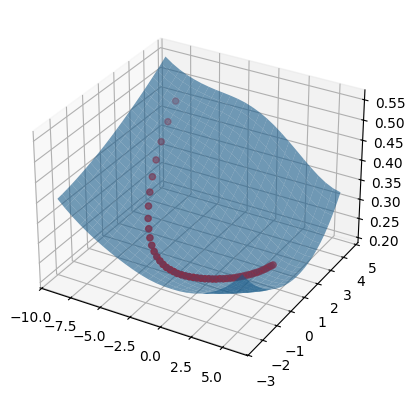
\includegraphics{CS541_HW3_git_files/figure-latex/cs541_hw3_p2-3_d1a-prob3-output-1.png}

}

\caption{Visualization of the loss landscape and optimization
trajectory.}

\end{figure}%

\begin{center}\rule{0.5\linewidth}{0.5pt}\end{center}

\section{Problem 4: Autoencoder (20
points)}\label{problem-4-autoencoder-20-points}

This assignment explores one powerful concept in deep learning:
\textbf{unsupervised representation learning with autoencoders}. You
will build a neural network that learns to compress and then reconstruct
images, forcing it to learn a meaningful representation of the data in
the process.

\subsection{Task 1: Data Preparation (2
point)}\label{task-1-data-preparation-2-point}

\begin{enumerate}
\def\labelenumi{\arabic{enumi}.}
\tightlist
\item
  Load the \textbf{Fashion MNIST} dataset using
  \texttt{torchvision.datasets.FashionMNIST}.
\item
  Use \texttt{torchvision.transforms.ToTensor} to convert the images to
  PyTorch tensors and normalize the pixel values to be in the range
  \([0.0, 1.0]\).
\item
  Create a \texttt{DataLoader} for both the training and test sets. For
  this unsupervised task, we only need the image data, not the labels.
\end{enumerate}

\begin{center}\rule{0.5\linewidth}{0.5pt}\end{center}

\subsection{Answer}\label{answer-8}

\begin{Shaded}
\begin{Highlighting}[]
\CommentTok{\# Task 1}

\KeywordTok{def}\NormalTok{ prepare\_data(batch\_size: }\BuiltInTok{int} \OperatorTok{=} \DecValTok{128}\NormalTok{):}
\NormalTok{    transform }\OperatorTok{=}\NormalTok{ transforms.ToTensor()  }\CommentTok{\# 28x28 grayscale {-}\textgreater{} float tensor in [0,1]}

\NormalTok{    train\_set }\OperatorTok{=}\NormalTok{ torchvision.datasets.FashionMNIST(}
\NormalTok{        root}\OperatorTok{=}\StringTok{"./"}\NormalTok{, train}\OperatorTok{=}\VariableTok{True}\NormalTok{, download}\OperatorTok{=}\VariableTok{True}\NormalTok{, transform}\OperatorTok{=}\NormalTok{transform}
\NormalTok{    )}
\NormalTok{    test\_set }\OperatorTok{=}\NormalTok{ torchvision.datasets.FashionMNIST(}
\NormalTok{        root}\OperatorTok{=}\StringTok{"./"}\NormalTok{, train}\OperatorTok{=}\VariableTok{False}\NormalTok{, download}\OperatorTok{=}\VariableTok{True}\NormalTok{, transform}\OperatorTok{=}\NormalTok{transform}
\NormalTok{    )}

\NormalTok{    train\_loader }\OperatorTok{=}\NormalTok{ DataLoader(train\_set, batch\_size}\OperatorTok{=}\NormalTok{batch\_size, shuffle}\OperatorTok{=}\VariableTok{True}\NormalTok{, num\_workers}\OperatorTok{=}\DecValTok{2}\NormalTok{)}
\NormalTok{    test\_loader  }\OperatorTok{=}\NormalTok{ DataLoader(test\_set,  batch\_size}\OperatorTok{=}\NormalTok{batch\_size, shuffle}\OperatorTok{=}\VariableTok{False}\NormalTok{, num\_workers}\OperatorTok{=}\DecValTok{2}\NormalTok{)}

    \CommentTok{\# quick checks}
    \BuiltInTok{print}\NormalTok{(}\StringTok{"n/Data ready"}\NormalTok{)}
    \BuiltInTok{print}\NormalTok{(}\SpecialStringTok{f"{-} train samples: }\SpecialCharTok{\{}\BuiltInTok{len}\NormalTok{(train\_set)}\SpecialCharTok{\}}\SpecialStringTok{"}\NormalTok{)}
    \BuiltInTok{print}\NormalTok{(}\SpecialStringTok{f"{-} test samples : }\SpecialCharTok{\{}\BuiltInTok{len}\NormalTok{(test\_set)}\SpecialCharTok{\}}\SpecialStringTok{"}\NormalTok{)}
    \BuiltInTok{print}\NormalTok{(}\SpecialStringTok{f"{-} image shape  : }\SpecialCharTok{\{}\NormalTok{train\_set[}\DecValTok{0}\NormalTok{][}\DecValTok{0}\NormalTok{]}\SpecialCharTok{.}\NormalTok{shape}\SpecialCharTok{\}}\SpecialStringTok{"}\NormalTok{)  }\CommentTok{\# (1, 28, 28)}
    \BuiltInTok{print}\NormalTok{(}\SpecialStringTok{f"{-} train batches: }\SpecialCharTok{\{}\BuiltInTok{len}\NormalTok{(train\_loader)}\SpecialCharTok{\}}\SpecialStringTok{"}\NormalTok{)}
    \ControlFlowTok{return}\NormalTok{ train\_loader, test\_loader}

\CommentTok{\# run task 1}
\NormalTok{train\_loader, test\_loader }\OperatorTok{=}\NormalTok{ prepare\_data(batch\_size}\OperatorTok{=}\DecValTok{128}\NormalTok{)}
\end{Highlighting}
\end{Shaded}

\phantomsection\label{task1}
\begin{verbatim}
n/Data ready
- train samples: 60000
- test samples : 10000
- image shape  : torch.Size([1, 28, 28])
- train batches: 469
\end{verbatim}

\begin{center}\rule{0.5\linewidth}{0.5pt}\end{center}

\subsection{Task 2: Autoencoder Architecture (6
points)}\label{task-2-autoencoder-architecture-6-points}

Construct a \textbf{dense autoencoder model} by creating a class that
inherits from \texttt{torch.nn.Module}. The model should consist of an
\textbf{encoder} and a \textbf{decoder} with the following symmetric
architecture:

\begin{itemize}
\item
  \textbf{An Encoder} that takes a flattened 784-dimensional input and
  maps it to a compressed representation.

  \begin{itemize}
  \tightlist
  \item
    Input layer (implicitly defined by the input shape).
  \item
    Dense layer (\texttt{nn.Linear}) with \textbf{128 units} followed by
    a \textbf{ReLU} activation (\texttt{nn.ReLU}).
  \item
    Dense layer with \textbf{64 units} followed by a \textbf{ReLU}
    activation. This layer's output is the \textbf{latent
    representation}, also known as the ``\textbf{bottleneck}''.
  \end{itemize}
\item
  \textbf{A Decoder} that takes the 64-dimensional latent representation
  and reconstructs the 784-dimensional image.

  \begin{itemize}
  \tightlist
  \item
    Dense layer with \textbf{128 units} followed by a \textbf{ReLU}
    activation.
  \item
    Dense layer with \textbf{784 units} followed by a \textbf{Sigmoid}
    activation (\texttt{nn.Sigmoid}). The sigmoid activation ensures the
    output values are in the range \([0.0, 1.0]\), matching the
    normalized input data.
  \end{itemize}
\end{itemize}

\begin{center}\rule{0.5\linewidth}{0.5pt}\end{center}

\subsection{Answer}\label{answer-9}

\begin{Shaded}
\begin{Highlighting}[]
\CommentTok{\# Task 2}

\KeywordTok{class}\NormalTok{ Autoencoder(nn.Module):}
    \KeywordTok{def} \FunctionTok{\_\_init\_\_}\NormalTok{(}\VariableTok{self}\NormalTok{):}
        \BuiltInTok{super}\NormalTok{().}\FunctionTok{\_\_init\_\_}\NormalTok{()}
        \VariableTok{self}\NormalTok{.encoder }\OperatorTok{=}\NormalTok{ nn.Sequential(}
\NormalTok{            nn.Linear(}\DecValTok{784}\NormalTok{, }\DecValTok{128}\NormalTok{), nn.ReLU(),}
\NormalTok{            nn.Linear(}\DecValTok{128}\NormalTok{, }\DecValTok{64}\NormalTok{),  nn.ReLU(),}
\NormalTok{        )}
        \VariableTok{self}\NormalTok{.decoder }\OperatorTok{=}\NormalTok{ nn.Sequential(}
\NormalTok{            nn.Linear(}\DecValTok{64}\NormalTok{, }\DecValTok{128}\NormalTok{),  nn.ReLU(),}
\NormalTok{            nn.Linear(}\DecValTok{128}\NormalTok{, }\DecValTok{784}\NormalTok{), nn.Sigmoid(),  }\CommentTok{\# keep outputs in [0,1]}
\NormalTok{        )}

    \KeywordTok{def}\NormalTok{ forward(}\VariableTok{self}\NormalTok{, x: torch.Tensor) }\OperatorTok{{-}\textgreater{}}\NormalTok{ torch.Tensor:}
        \ControlFlowTok{return} \VariableTok{self}\NormalTok{.decoder(}\VariableTok{self}\NormalTok{.encoder(x))}

    \KeywordTok{def}\NormalTok{ encode(}\VariableTok{self}\NormalTok{, x: torch.Tensor) }\OperatorTok{{-}\textgreater{}}\NormalTok{ torch.Tensor:}
        \ControlFlowTok{return} \VariableTok{self}\NormalTok{.encoder(x)}

\CommentTok{\# build model and show size}
\NormalTok{model }\OperatorTok{=}\NormalTok{ Autoencoder()}
\NormalTok{params }\OperatorTok{=} \BuiltInTok{sum}\NormalTok{(p.numel() }\ControlFlowTok{for}\NormalTok{ p }\KeywordTok{in}\NormalTok{ model.parameters())}
\BuiltInTok{print}\NormalTok{(}\StringTok{"Model ready"}\NormalTok{)}
\BuiltInTok{print}\NormalTok{(}\SpecialStringTok{f"{-} parameters: }\SpecialCharTok{\{}\NormalTok{params}\SpecialCharTok{:,\}}\SpecialStringTok{"}\NormalTok{)}

\end{Highlighting}
\end{Shaded}

\phantomsection\label{task2}
\begin{verbatim}
Model ready
- parameters: 218,192
\end{verbatim}

\begin{center}\rule{0.5\linewidth}{0.5pt}\end{center}

\subsection{Task 3: Model Training (6
points)}\label{task-3-model-training-6-points}

\begin{enumerate}
\def\labelenumi{\arabic{enumi}.}
\tightlist
\item
  Instantiate your model, a loss function (\texttt{nn.MSELoss} is a good
  choice), and an optimizer (\texttt{torch.optim.Adam}).
\item
  Write a training loop that iterates for \textbf{20 epochs}. In each
  epoch, iterate through the training \texttt{DataLoader}.
\item
  For each batch of images, you must:

  \begin{itemize}
  \tightlist
  \item
    Flatten the \(28\times28\) images into 784-dimensional vectors.
  \item
    Perform a forward pass to get the reconstructed images.
  \item
    Calculate the loss between the original and reconstructed images.
  \item
    Zero the gradients, perform a backward pass, and update the weights.
  \end{itemize}
\end{enumerate}

\begin{center}\rule{0.5\linewidth}{0.5pt}\end{center}

\subsection{Answer}\label{answer-10}

\begin{Shaded}
\begin{Highlighting}[]
\CommentTok{\# Task 3}

\KeywordTok{def}\NormalTok{ train\_autoencoder(model: nn.Module, loader: DataLoader, epochs: }\BuiltInTok{int} \OperatorTok{=} \DecValTok{20}\NormalTok{, lr: }\BuiltInTok{float} \OperatorTok{=} \FloatTok{1e{-}3}\NormalTok{):}
\NormalTok{    device }\OperatorTok{=}\NormalTok{ torch.device(}\StringTok{"cuda"} \ControlFlowTok{if}\NormalTok{ torch.cuda.is\_available() }\ControlFlowTok{else} \StringTok{"cpu"}\NormalTok{)}
\NormalTok{    model }\OperatorTok{=}\NormalTok{ model.to(device)}
\NormalTok{    opt }\OperatorTok{=}\NormalTok{ optim.Adam(model.parameters(), lr}\OperatorTok{=}\NormalTok{lr)}
\NormalTok{    loss\_fn }\OperatorTok{=}\NormalTok{ nn.MSELoss()}

    \BuiltInTok{print}\NormalTok{(}\SpecialStringTok{f"Training on }\SpecialCharTok{\{}\NormalTok{device}\SpecialCharTok{\}}\SpecialStringTok{ for }\SpecialCharTok{\{}\NormalTok{epochs}\SpecialCharTok{\}}\SpecialStringTok{ epochs"}\NormalTok{)}
\NormalTok{    losses }\OperatorTok{=}\NormalTok{ []}

    \ControlFlowTok{for}\NormalTok{ epoch }\KeywordTok{in} \BuiltInTok{range}\NormalTok{(}\DecValTok{1}\NormalTok{, epochs }\OperatorTok{+} \DecValTok{1}\NormalTok{):}
\NormalTok{        model.train()}
\NormalTok{        running }\OperatorTok{=} \FloatTok{0.0}

        \ControlFlowTok{for}\NormalTok{ i, (imgs, \_) }\KeywordTok{in} \BuiltInTok{enumerate}\NormalTok{(loader):}
\NormalTok{            imgs }\OperatorTok{=}\NormalTok{ imgs.to(device).view(imgs.size(}\DecValTok{0}\NormalTok{), }\OperatorTok{{-}}\DecValTok{1}\NormalTok{)   }\CommentTok{\# (B, 1, 28, 28) {-}\textgreater{} (B, 784)}

\NormalTok{            opt.zero\_grad()}
\NormalTok{            out }\OperatorTok{=}\NormalTok{ model(imgs)}
\NormalTok{            loss }\OperatorTok{=}\NormalTok{ loss\_fn(out, imgs)}
\NormalTok{            loss.backward()}
\NormalTok{            opt.step()}

\NormalTok{            running }\OperatorTok{+=}\NormalTok{ loss.item()}
            \ControlFlowTok{if}\NormalTok{ i }\OperatorTok{\%} \DecValTok{100} \OperatorTok{==} \DecValTok{0}\NormalTok{:}
                \BuiltInTok{print}\NormalTok{(}\SpecialStringTok{f"  epoch }\SpecialCharTok{\{}\NormalTok{epoch}\SpecialCharTok{:2d\}}\SpecialStringTok{ | batch }\SpecialCharTok{\{}\NormalTok{i}\SpecialCharTok{:4d\}}\SpecialStringTok{/}\SpecialCharTok{\{}\BuiltInTok{len}\NormalTok{(loader)}\SpecialCharTok{\}}\SpecialStringTok{ | loss }\SpecialCharTok{\{}\NormalTok{loss}\SpecialCharTok{.}\NormalTok{item()}\SpecialCharTok{:.4f\}}\SpecialStringTok{"}\NormalTok{)}

\NormalTok{        avg }\OperatorTok{=}\NormalTok{ running }\OperatorTok{/} \BuiltInTok{len}\NormalTok{(loader)}
\NormalTok{        losses.append(avg)}
        \BuiltInTok{print}\NormalTok{(}\SpecialStringTok{f"  epoch }\SpecialCharTok{\{}\NormalTok{epoch}\SpecialCharTok{:2d\}}\SpecialStringTok{ complete | avg loss }\SpecialCharTok{\{}\NormalTok{avg}\SpecialCharTok{:.4f\}}\SpecialStringTok{"}\NormalTok{)}

    \ControlFlowTok{return}\NormalTok{ model, losses}

\CommentTok{\# run task 3}
\NormalTok{model, losses }\OperatorTok{=}\NormalTok{ train\_autoencoder(model, train\_loader, epochs}\OperatorTok{=}\DecValTok{20}\NormalTok{, lr}\OperatorTok{=}\FloatTok{1e{-}3}\NormalTok{)}
\end{Highlighting}
\end{Shaded}

\phantomsection\label{task3}
\begin{verbatim}
Training on cuda for 20 epochs
  epoch  1 | batch    0/469 | loss 0.1714
  epoch  1 | batch  100/469 | loss 0.0410
  epoch  1 | batch  200/469 | loss 0.0289
  epoch  1 | batch  300/469 | loss 0.0250
  epoch  1 | batch  400/469 | loss 0.0228
  epoch  1 complete | avg loss 0.0374
  epoch  2 | batch    0/469 | loss 0.0212
  epoch  2 | batch  100/469 | loss 0.0196
  epoch  2 | batch  200/469 | loss 0.0210
  epoch  2 | batch  300/469 | loss 0.0218
  epoch  2 | batch  400/469 | loss 0.0195
  epoch  2 complete | avg loss 0.0198
  epoch  3 | batch    0/469 | loss 0.0173
  epoch  3 | batch  100/469 | loss 0.0168
  epoch  3 | batch  200/469 | loss 0.0161
  epoch  3 | batch  300/469 | loss 0.0163
  epoch  3 | batch  400/469 | loss 0.0155
  epoch  3 complete | avg loss 0.0172
  epoch  4 | batch    0/469 | loss 0.0167
  epoch  4 | batch  100/469 | loss 0.0159
  epoch  4 | batch  200/469 | loss 0.0151
  epoch  4 | batch  300/469 | loss 0.0149
  epoch  4 | batch  400/469 | loss 0.0153
  epoch  4 complete | avg loss 0.0156
  epoch  5 | batch    0/469 | loss 0.0158
  epoch  5 | batch  100/469 | loss 0.0156
  epoch  5 | batch  200/469 | loss 0.0147
  epoch  5 | batch  300/469 | loss 0.0141
  epoch  5 | batch  400/469 | loss 0.0151
  epoch  5 complete | avg loss 0.0145
  epoch  6 | batch    0/469 | loss 0.0133
  epoch  6 | batch  100/469 | loss 0.0143
  epoch  6 | batch  200/469 | loss 0.0126
  epoch  6 | batch  300/469 | loss 0.0132
  epoch  6 | batch  400/469 | loss 0.0135
  epoch  6 complete | avg loss 0.0136
  epoch  7 | batch    0/469 | loss 0.0130
  epoch  7 | batch  100/469 | loss 0.0145
  epoch  7 | batch  200/469 | loss 0.0117
  epoch  7 | batch  300/469 | loss 0.0120
  epoch  7 | batch  400/469 | loss 0.0115
  epoch  7 complete | avg loss 0.0129
  epoch  8 | batch    0/469 | loss 0.0125
  epoch  8 | batch  100/469 | loss 0.0124
  epoch  8 | batch  200/469 | loss 0.0116
  epoch  8 | batch  300/469 | loss 0.0124
  epoch  8 | batch  400/469 | loss 0.0126
  epoch  8 complete | avg loss 0.0124
  epoch  9 | batch    0/469 | loss 0.0135
  epoch  9 | batch  100/469 | loss 0.0118
  epoch  9 | batch  200/469 | loss 0.0108
  epoch  9 | batch  300/469 | loss 0.0125
  epoch  9 | batch  400/469 | loss 0.0126
  epoch  9 complete | avg loss 0.0119
  epoch 10 | batch    0/469 | loss 0.0112
  epoch 10 | batch  100/469 | loss 0.0115
  epoch 10 | batch  200/469 | loss 0.0111
  epoch 10 | batch  300/469 | loss 0.0117
  epoch 10 | batch  400/469 | loss 0.0115
  epoch 10 complete | avg loss 0.0116
  epoch 11 | batch    0/469 | loss 0.0104
  epoch 11 | batch  100/469 | loss 0.0115
  epoch 11 | batch  200/469 | loss 0.0109
  epoch 11 | batch  300/469 | loss 0.0115
  epoch 11 | batch  400/469 | loss 0.0108
  epoch 11 complete | avg loss 0.0112
  epoch 12 | batch    0/469 | loss 0.0111
  epoch 12 | batch  100/469 | loss 0.0114
  epoch 12 | batch  200/469 | loss 0.0109
  epoch 12 | batch  300/469 | loss 0.0108
  epoch 12 | batch  400/469 | loss 0.0099
  epoch 12 complete | avg loss 0.0109
  epoch 13 | batch    0/469 | loss 0.0110
  epoch 13 | batch  100/469 | loss 0.0109
  epoch 13 | batch  200/469 | loss 0.0101
  epoch 13 | batch  300/469 | loss 0.0124
  epoch 13 | batch  400/469 | loss 0.0093
  epoch 13 complete | avg loss 0.0107
  epoch 14 | batch    0/469 | loss 0.0113
  epoch 14 | batch  100/469 | loss 0.0112
  epoch 14 | batch  200/469 | loss 0.0105
  epoch 14 | batch  300/469 | loss 0.0104
  epoch 14 | batch  400/469 | loss 0.0102
  epoch 14 complete | avg loss 0.0105
  epoch 15 | batch    0/469 | loss 0.0115
  epoch 15 | batch  100/469 | loss 0.0096
  epoch 15 | batch  200/469 | loss 0.0098
  epoch 15 | batch  300/469 | loss 0.0101
  epoch 15 | batch  400/469 | loss 0.0123
  epoch 15 complete | avg loss 0.0103
  epoch 16 | batch    0/469 | loss 0.0100
  epoch 16 | batch  100/469 | loss 0.0114
  epoch 16 | batch  200/469 | loss 0.0111
  epoch 16 | batch  300/469 | loss 0.0105
  epoch 16 | batch  400/469 | loss 0.0103
  epoch 16 complete | avg loss 0.0101
  epoch 17 | batch    0/469 | loss 0.0092
  epoch 17 | batch  100/469 | loss 0.0106
  epoch 17 | batch  200/469 | loss 0.0095
  epoch 17 | batch  300/469 | loss 0.0099
  epoch 17 | batch  400/469 | loss 0.0101
  epoch 17 complete | avg loss 0.0100
  epoch 18 | batch    0/469 | loss 0.0099
  epoch 18 | batch  100/469 | loss 0.0101
  epoch 18 | batch  200/469 | loss 0.0093
  epoch 18 | batch  300/469 | loss 0.0105
  epoch 18 | batch  400/469 | loss 0.0097
  epoch 18 complete | avg loss 0.0098
  epoch 19 | batch    0/469 | loss 0.0101
  epoch 19 | batch  100/469 | loss 0.0104
  epoch 19 | batch  200/469 | loss 0.0094
  epoch 19 | batch  300/469 | loss 0.0089
  epoch 19 | batch  400/469 | loss 0.0085
  epoch 19 complete | avg loss 0.0097
  epoch 20 | batch    0/469 | loss 0.0097
  epoch 20 | batch  100/469 | loss 0.0088
  epoch 20 | batch  200/469 | loss 0.0108
  epoch 20 | batch  300/469 | loss 0.0094
  epoch 20 | batch  400/469 | loss 0.0093
  epoch 20 complete | avg loss 0.0095
\end{verbatim}

\begin{center}\rule{0.5\linewidth}{0.5pt}\end{center}

\subsection{Task 4: Visualizing Reconstructions (6
points)}\label{task-4-visualizing-reconstructions-6-points}

\begin{enumerate}
\def\labelenumi{\arabic{enumi}.}
\tightlist
\item
  Set your model to \textbf{evaluation mode}.
\item
  Get a batch of images from the test set and pass them through your
  trained autoencoder to get the reconstructions.
\item
  Create a plot showing \textbf{two different original images} from the
  test set and their corresponding reconstructions directly below them.
\item
  \textbf{Deliverable:} A single figure containing 4 images (2 original
  test images, 2 reconstructed images), clearly labeled.
\end{enumerate}

\begin{center}\rule{0.5\linewidth}{0.5pt}\end{center}

\subsection{Answer}\label{answer-11}

\begin{Shaded}
\begin{Highlighting}[]
\CommentTok{\# Task 4}

\KeywordTok{def}\NormalTok{ visualize\_reconstructions(model: nn.Module, test\_loader: DataLoader, num\_images: }\BuiltInTok{int} \OperatorTok{=} \DecValTok{2}\NormalTok{):}
\NormalTok{    model.}\BuiltInTok{eval}\NormalTok{()}
\NormalTok{    device }\OperatorTok{=} \BuiltInTok{next}\NormalTok{(model.parameters()).device}

\NormalTok{    images, \_ }\OperatorTok{=} \BuiltInTok{next}\NormalTok{(}\BuiltInTok{iter}\NormalTok{(test\_loader))}
\NormalTok{    images }\OperatorTok{=}\NormalTok{ images.to(device)}
    \ControlFlowTok{with}\NormalTok{ torch.no\_grad():}
\NormalTok{        recon }\OperatorTok{=}\NormalTok{ model(images.view(images.size(}\DecValTok{0}\NormalTok{), }\OperatorTok{{-}}\DecValTok{1}\NormalTok{)).view(}\OperatorTok{{-}}\DecValTok{1}\NormalTok{, }\DecValTok{1}\NormalTok{, }\DecValTok{28}\NormalTok{, }\DecValTok{28}\NormalTok{)}

\NormalTok{    images }\OperatorTok{=}\NormalTok{ images.cpu()}
\NormalTok{    recon }\OperatorTok{=}\NormalTok{ recon.cpu()}

\NormalTok{    fig, axes }\OperatorTok{=}\NormalTok{ plt.subplots(}\DecValTok{2}\NormalTok{, }\DecValTok{2}\NormalTok{, figsize}\OperatorTok{=}\NormalTok{(}\DecValTok{8}\NormalTok{, }\DecValTok{4}\NormalTok{))}
\NormalTok{    axes[}\DecValTok{0}\NormalTok{, }\DecValTok{0}\NormalTok{].imshow(images[}\DecValTok{0}\NormalTok{].squeeze(), cmap}\OperatorTok{=}\StringTok{"gray"}\NormalTok{)}\OperatorTok{;}\NormalTok{ axes[}\DecValTok{0}\NormalTok{, }\DecValTok{0}\NormalTok{].set\_title(}\StringTok{"Original 1"}\NormalTok{)}\OperatorTok{;}\NormalTok{ axes[}\DecValTok{0}\NormalTok{, }\DecValTok{0}\NormalTok{].axis(}\StringTok{"off"}\NormalTok{)}
\NormalTok{    axes[}\DecValTok{1}\NormalTok{, }\DecValTok{0}\NormalTok{].imshow(recon[}\DecValTok{0}\NormalTok{].squeeze(),   cmap}\OperatorTok{=}\StringTok{"gray"}\NormalTok{)}\OperatorTok{;}\NormalTok{ axes[}\DecValTok{1}\NormalTok{, }\DecValTok{0}\NormalTok{].set\_title(}\StringTok{"Reconstructed 1"}\NormalTok{)}\OperatorTok{;}\NormalTok{ axes[}\DecValTok{1}\NormalTok{, }\DecValTok{0}\NormalTok{].axis(}\StringTok{"off"}\NormalTok{)}
\NormalTok{    axes[}\DecValTok{0}\NormalTok{, }\DecValTok{1}\NormalTok{].imshow(images[}\DecValTok{1}\NormalTok{].squeeze(), cmap}\OperatorTok{=}\StringTok{"gray"}\NormalTok{)}\OperatorTok{;}\NormalTok{ axes[}\DecValTok{0}\NormalTok{, }\DecValTok{1}\NormalTok{].set\_title(}\StringTok{"Original 2"}\NormalTok{)}\OperatorTok{;}\NormalTok{ axes[}\DecValTok{0}\NormalTok{, }\DecValTok{1}\NormalTok{].axis(}\StringTok{"off"}\NormalTok{)}
\NormalTok{    axes[}\DecValTok{1}\NormalTok{, }\DecValTok{1}\NormalTok{].imshow(recon[}\DecValTok{1}\NormalTok{].squeeze(),   cmap}\OperatorTok{=}\StringTok{"gray"}\NormalTok{)}\OperatorTok{;}\NormalTok{ axes[}\DecValTok{1}\NormalTok{, }\DecValTok{1}\NormalTok{].set\_title(}\StringTok{"Reconstructed 2"}\NormalTok{)}\OperatorTok{;}\NormalTok{ axes[}\DecValTok{1}\NormalTok{, }\DecValTok{1}\NormalTok{].axis(}\StringTok{"off"}\NormalTok{)}
\NormalTok{    fig.suptitle(}\StringTok{"Autoencoder: Test Originals vs Reconstructions"}\NormalTok{)}
\NormalTok{    plt.tight\_layout()}
\NormalTok{    plt.show()}

\CommentTok{\# run task 4}
\NormalTok{visualize\_reconstructions(model, test\_loader, num\_images}\OperatorTok{=}\DecValTok{2}\NormalTok{)}

\end{Highlighting}
\end{Shaded}

\begin{figure}[H]

{\centering 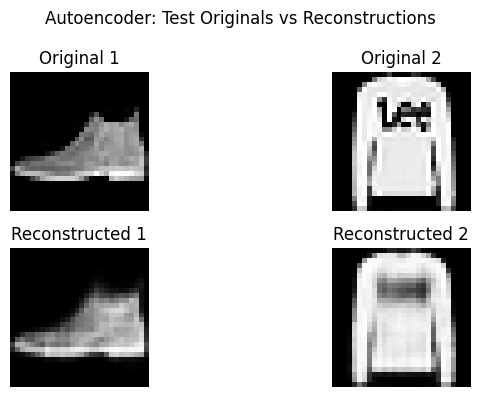
\includegraphics{CS541_HW3_git_files/figure-latex/cs541_hw3_p4_d1a-task4-output-1.png}

}

\caption{Autoencoder reconstructions on test set: Originals (top) vs
Reconstructions (bottom).}

\end{figure}%

\begin{center}\rule{0.5\linewidth}{0.5pt}\end{center}

\section{Submission}\label{submission}

Submit one PDF file that includes your notes for the theoretical
problems (scanned or typed) and screenshots of your code for the
programming problems. All material in the submitted PDF must be
presented in a clear and readable format.

If you are working as part of a group, then indicate the members on
canvas:
\href{https://www.google.com/search?q=https://canvas.wpi.edu/courses/76771/groups\%23tab-14853}{https://canvas.wpi.edu/courses/76771/groups\#tab-14853}.
Once you do that, be aware that any submission from a team member will
overwrite an existing one.

\subsection{Teamwork}\label{teamwork}

You may complete this homework assignment either individually or in
teams up to 2 people.




\end{document}
